\documentclass[12pt,openright,twoside,a4paper,english,french,spanish]{abntex2}

\usepackage{cmap}
\usepackage{lmodern}
\usepackage[T1]{fontenc}
\usepackage[utf8]{inputenc}
\usepackage{lastpage}
\usepackage{indentfirst}
\usepackage{color}
\usepackage{graphicx}
\usepackage{units}
\usepackage[brazilian,hyperpageref]{backref}
\usepackage[alf]{abntex2cite}
\usepackage{bold-extra}
\usepackage{eso-pic}
\usepackage{gensymb}
\usepackage{listings}
\usepackage{color}
\usepackage{caption}
\usepackage{subcaption}
\usepackage{mathtools}
\usepackage{array}
\usepackage{multirow}
\usepackage[table,xcdraw]{xcolor}
\usepackage{longtable}
\usepackage{url}
\usepackage{imakeidx}

\newcolumntype{t}{>{\arraybackslash}m{10cm}}
\newcolumntype{y}{>{\arraybackslash}m{7cm}}
\newcolumntype{u}{>{\arraybackslash}m{7cm}}

\definecolor{codegreen}{rgb}{0,0.6,0}
\definecolor{red}{rgb}{1,0,0}
\definecolor{codegray}{rgb}{0.5,0.5,0.5}
\definecolor{codepurple}{rgb}{0.58,0,0.82}
\definecolor{backcolour}{rgb}{0.98,0.98,0.95}

\lstdefinestyle{mystyle}{
    backgroundcolor=\color{backcolour},
    commentstyle=\color{codegreen},
    keywordstyle=\color{magenta},
    numberstyle=\tiny\color{codegray},
    stringstyle=\color{codepurple},
    basicstyle=\footnotesize,
    breakatwhitespace=false,
    breaklines=true,
    captionpos=b,
    keepspaces=true,
    numbers=left,
    numbersep=5pt,
    showspaces=false,
    showstringspaces=false,
    showtabs=false,
    tabsize=2
}

\lstset{style=mystyle,literate=%
    {à}{{\`a}}1
    {ã}{{\~a}}1
}


\input{fixos/comandos}
\input{fixos/novosComandos}

% Dados pessoais
\autor{Matheus Souza Fernandes}
\curso{Engenharia de Software}

% Dados do trabalho
\titulo{Tenho Dito: uma aplicação para análise de discursos parlamentares utilizando técnicas de processamento de linguagem natural}
\data{2016}
\palavraChaveUm{processamento de linguagem natural}
\palavraChaveDois{aprendizado de máquina}

% Dados da orientacao
\orientador{Prof. Dr. Fábio Macedo Mendes}
\coorientador{}

% Dados para a ficha catalográfica
\cdu{02:141:005.6}

% Dados da aprovação do trabalho
\dataDaAprovacao{01 de junho de 2013}
\membroConvidadoUm{Prof. Dr. Paulo Roberto Miranda Meirelles}
\membroConvidadoDois{Prof. Dr. Teófilo de Campos}

% Dados pessoais
\autor{Matheus Souza Fernandes}
\curso{Engenharia de Software}

% Dados do trabalho
\titulo{Tenho Dito: uma aplicação para análise de discursos parlamentares utilizando técnicas de processamento de linguagem natural}
\data{2016}
\palavraChaveUm{processamento de linguagem natural}
\palavraChaveDois{aprendizado de máquina}

% Dados da orientacao
\orientador{Prof. Dr. Fábio Macedo Mendes}
\coorientador{}

% Dados para a ficha catalográfica
\cdu{02:141:005.6}

% Dados da aprovação do trabalho
\dataDaAprovacao{01 de junho de 2013}
\membroConvidadoUm{Prof. Dr. Paulo Roberto Miranda Meirelles}
\membroConvidadoDois{Prof. Dr. Teófilo de Campos}

\input{fixos/setup}

\indexsetup{level=\chapter}
\makeindex[name=urls, title={Links Importantes}, columns=1]
\newcommand{\lnk}[2]{#2\index[urls]{#1: \url{#2}}}

\begin{document}

\frenchspacing
\imprimircapa
\imprimirfolhaderosto*

\input{fixos/fichaCatalografica}
% \input{editaveis/errata}
\input{fixos/folhaDeAprovacao}
% \input{editaveis/dedicatoria}
% \begin{agradecimentos}

Primeiramente, agradeço a Deus por ter me dado força e saúde para chegar até aqui. Agradeço também aos meus pais e irmãos, pelo apoio e por não medirem esforços para que eu sempre tivesse boas condições de estudo.

Agradeço a Paola, minha noiva e companheira, que sempre me apoiou e me deu forças para continuar lutando, que nos momentos mais difíceis estava ao meu lado, com quem compatilho tudo e posso contar sempre. Obrigado por ser essa pessoa tão especial na minha vida, eu te amo.

Agradeço ao meu orientador, Fábio Mendes, pelo apoio, confiança e paciência de me passar um pouco de seus conhecimentos. Agradeço também aos membros da banca, Paulo e Téo, pelas críticas construtivas e orientações.

Agradeço a todos os amigos do Laboratório Hacker, pelo carinho, apoio no desenvolvimento desse trabalho e compreensão pela ausência nos happy hours.

Agradeço a todos os professores que fizeram parte da minha graduação e ajudaram a formar o profissional que sou hoje.

Agradeço a todo o pessoal do LAPPIS e companheiros de curso pela incrível troca de conhecimentos e, claro, pelo bullying educativo. Agradeço também pelas amizades criadas durante todos esses anos.


\end{agradecimentos}

% \input{editaveis/epigrafe}
\begin{resumo}
O processamento de linguagem natural tem sido utilizado com sucesso na área de análise de discurso, onde é possível reconhecer padrões e classificar textos, extraindo informações de grandes volumes de dados. Este trabalho tem como objetivo extrair o perfil temático dos deputados federais, através do processamento dos textos obtidos de seus discursos e proposições, bem como desenvolver uma aplicação \textit{web} para que os resultados dessa pesquisa sejam apresentados de forma lúdica e amigável. O texto discute as técnicas de processamento de linguagem natural utilizadas nesta análise, que incluem a remoção de \textit{stop words}, algumas técnicas de \textit{stemização}, representação dos textos em \textit{bag-of-words} e algumas técnicas de aprendizagem de máquina supervisionada e não-supervisionada, como \textit{Naive Bayes} e \(k\)-means.

 \vspace{\onelineskip}

 \noindent
 \textbf{Palavras-chaves}: Processamento de linguagem natural, aprendizado de máquina.
\end{resumo}

\begin{resumo}[Abstract]
 \begin{otherlanguage*}{english}
   Natural language processing has been used successfully in the discourse analysis where it's possible to recognize patterns and classify texts, extracting information from large volume of data. This paper aim to extract the thematic profile of the federal deputies through the processing of texts obteined from their speeches and proposals, as well as develop a web application so that the results of this research are presented in a playful and friendly way. The text discusses the natural language processing techniques used in this analysis, which include the removal of stop words, some stemming techniques, representation of texts in bag-of-words model and some techniques of supervisioned and unsupervisioned machine learning, such as Naive Bayes and k-means.

   \vspace{\onelineskip}

   \noindent
   \textbf{Key-words}: Natural language processing, machine learning.
 \end{otherlanguage*}
\end{resumo}

\input{fixos/listasAutomaticas}
% \input{editaveis/abreviaturas}
% \input{editaveis/simbolos}
\input{fixos/indiceAutomatico}

\textual

\chapter{Introdução}

\section{Contextualização}
\label{sec:contextualização}

O desenvolvimento de novas ferramentas de interação entre governo e sociedade é fundamental para o avanço da democracia e a disponibilização de dados governamentais possibilita que novas aplicações surjam, trazendo novas formas de utilização e interpretação destes dados \cite{consegi2011}. O presente trabalho utiliza dados disponíveis publicamente pela Câmara dos Deputados Federal para analisar textos de discursos e proposições parlamentares utilizando técnicas de processamento de linguagem natural e aprendizagem de máquina. O objetivo da análise é determinar eixos temáticos para cada deputado e avaliar o alinhamento entre os temas dos discursos e das propostas encaminhadas.

Com o objetivo de apresentar uma nova forma de visualizar os dados de discursos e proposições já disponibilizados pela Câmara dos Deputados, esse trabalho terá como produto um sistema \textit{web} onde será possível, através de gráficos interativos, conhecer o perfil temático dos deputados federais. Para chegar à esse perfil, foram utilizadas técnicas de processamento de linguagem natural e aprendizado de máquina, como classificadores \textit{naive Bayes}, por exemplo.

No contexto governamental, os Dados Abertos\footnote{O conceito para Dado Aberto considerado neste trabalho é o definido pela \citeonline{open_knowledge}, que estabele que um dado (ou um conhecimento) é aberto quando estiver livre para uso, reuso e redistribuição. Ou seja, a informação deve estar disponível a todos, sem restrições de \textit{copyright}, patentes ou outros mecanismos de controle. Além disso, esses dados devem ser independentes de tecnologia, baseados em formatos padronizados e desvinculados das ferramentas que os originaram. Os dados devem permitir sua manipulação por máquinas e possuir metadados que permitam identificar sua natureza, origem e qualidade \cite{diniz2010}.} fortalecem três características indispensáveis para a democracia: transparência, participação e colaboração \cite{consegi2011}. Transparência tem o papel de informar a sociedade sobre as ações que estão sendo tomadas ou que serão tomadas pelo governo. Participação permite que os cidadãos auxiliem o poder público a elaborar políticas mais eficazes. Finalmente, a colaboração entre a sociedade, diferentes níveis de governo e a iniciativa privada permitem aprimorar a eficácia do Estado.

De acordo com a Lei n\degree 12.527/2011, também conhecida como Lei de Acesso à Informação, qualquer cidadão, sem necessidade de justificativa, pode solicitar dados ou informações à qualquer órgão ou entidade pública dos poderes Executivo, Legislativo e Judiciário, além do Ministério Público, nas esferas Federal, Estadual e Municipal \cite{lei_acesso_informacao}. Para atender à lei mencionada anteriormente, a \citeonline{camara_dados_abertos} criou um portal que tem como objetivo disponibilizar dados brutos para a utilização em aplicações desenvolvidas pelos cidadãos e entidades da sociedade civil que permitam a percepção mais efetiva das atividades parlamentares.

A publicação de dados pressupõe o uso de tecnologias que garantam que eles possam ser acessados e reutilizados por máquinas. Apesar de não garantir que os dados estarão disponíveis em um formato conveniente de uso imediato, possibilita o cruzamento de diferentes bases dados e a exibição destes de forma que possam ser melhor apresentados à sociedade \cite{diniz2010}.

\section{Objetivo}
\label{sec:objetivo}

O objetivo desse trabalho é utilizar técnicas de processamento de linguagem natural para, através da análise dos discursos e proposições dos parlamentares, determinar um perfil temático para os deputados, bem como evidenciar o termos mais utilizados em seus discursos e proposições e, assim, permitir que o cidadão veja, de forma comparativa, o que seus representantes no parlamento mais dizem em seus discursos e o que mais dizem em suas proposições.

\subsection{Contribuições Tecnológicas}
\label{sub:contribuicoes_tecnologicas}

\begin{itemize}
    \item Implementar biblioteca Python para consumo de dados abertos governamentais, com foco nos dados abertos da Câmara dos Deputados.
    \item Implementar aplicação Django para utilização e persistência dos dados abertos governamentais, também com foco nos dados aberto da Câmara dos Deputados.
    \item Implementar sistema web de comparação temática entre discursos e proposições parlamentares, a ser detalhado no decorrer deste trabalho.
\end{itemize}

\section{Metodologia}
\label{sub:metodologia}

Devido à natureza deste trabalho, nota-se que o modelo de pesquisa adequado deve possuir características tanto da pesquisa exploratória quanto da pesquisa experimental. Outro método de pesquisa que será utilizado é a pesquisa-ação, onde existirão ciclos de coleta e análise de dados. A cada ciclo, a análise dos dados do ciclo anterior servirão de insumo para tomadas de decisão no desenvolvimento do projeto.

O presente trabalho possui o apoio do Laboratório Hacker da Câmara dos Deputados e por isso foi desenvolvido em colaboração com membros de sua equipe de desenvolvimento. Para facilitar a interação com os outros envolvidos no projeto, foi criada uma organização no \textit{GitHub}\footnote{\lnk{- Organização do Tenho Dito no \textit{GitHub}}{https://github.com/tenhodito}}, onde foram armazenados os códigos produzidos nesse trabalho. Além disso, a aplicação será hopedada na infraestrutura do Laboratório Hacker.

Por motivos de força maior, o presente trabalho não foi completado até a data limite para sua entrega e a versão atualizada do texto poderá ser obtida no repositório do autor\footnote{\lnk{- Texto atualizado}{https://github.com/msfernandes/tcc}}, bem como a versão final do código poderá ser acessado no repositório do Tenho Dito\footnote{\lnk{- Repositório do Tenho Dito}{https://github.com/tenhodito/tenhodito}}.

\section{Organização do Trabalho}
\label{sec:organização_do_trabalho}

Esse trabalho está organizado em 5 capítulos: Introdução, Metodologia, Processamento de Linguagem Natural, Resultados Obtidos e Considreações Finais. O presente capítulo faz uma breve introdução ao tema desse trabalho, bem como aos objetivos que pretendem ser alcançados. O capítulo 2, Metodologia, descreve a forma como foi realizado esse trabalho. O capítulo 3 contém todas o referencial teórico necessário para a realização desse trabalho. O capítulo 4 expõe os objetivos alcançado ao final do trabalho. O capítulo 5 possui a conclusão a que se chega com o presente trabalho e as perspectivas futuras.

\clearpage
\chapter{Processamento de Linguagem Natural}

Este capítulo contém o referencial teórico que diz respeito ao Processamento de Linguagem Natural.

\section{Pré-processamento: modelo \textit{bag-of-words} (BOW)}
\label{sec:modelo_te}

A maior parte dos dados utilizados nesse trabalho estão dispostos em formato de texto, ou seja, um formato não estruturado que dificulta a extração de informações. Um método comum do processamento de texto em linguagem natural é o modelo \textit{bag-of-words}, onde o texto é representado na forma de um vetor de frequência de palavras \cite{pretext}.

A representação computacional de um texto no modelo mencionado é feita através de um dicionário onde suas chaves são os termos presentes no documento e os valores são as respectivas frequências. Tomando o trecho ``fui à padaria e comprei pão'' como exemplo, sua representação no modelo \textit{bag-of-words} corresponderia a:

\begin{lstlisting}[language=Python, caption=Representação de um trecho  no modelo bag-of-words]
bag_of_words = {
    "fui": 1,
    "à": 1,
    "padaria": 1,
    "e": 1,
    "comprei": 1,
    "pão": 1,
}
\end{lstlisting}

É fácil ver que esta representação torna a ordem das palavras irrelevante. As frases ``e comprei fui padaria pão à'' e ``à pão comprei padaria e fui'' também possuem as mesmas representações.

O texto também pode ser representado na forma de um vetor. Nesse caso, cada índice do vetor representa uma palavra e cada coordenada corresponde à frequência da mesma. Quando mais de um texto é analisado, os vetores que os representam devem possuir a mesma relação ``índice-palavra''. Por isso, as palavras que compõe cada texto são ordenadas alfbéticamente antes da formação do vetores.

A linguagem de programação \textit{Python} possui, nativamente, ferramentas que facilitam a contagem de elementos de um dicionário. O módulo \texttt{collections}\footnote{https://docs.python.org/3/library/collections.html} possui a classe \texttt{Counter}, que é uma subclasse de \texttt{dict} e representa um mapa entre elementos e números. Isso torna o \texttt{Counter} uma representação ideal para o modelo \textit{bag-of-words}, já que ele, naturalmente, conta a quantidade de vezes que um termo aparece dentro de uma coleção (uma lista, tupla ou dicionário, por exemplo).

\subsection{Valores no BOW}
\label{sec:representação_dos_termos}

Apresentamos o modelo do BOW associando um valor \(a_i\) a cada palavra que representa, como a quantidade de vezes que o termo aparece em um texto. Existem, no entanto, outras formas de representação expostas a seguir.

\subsubsection{\textit{Boolean}}
\label{ssub:bag-boolean}

Essa medida associa valores binários para os termos presentes nos documentos, onde o valor de \(a_{i}\) é 0 quando o termo não aparece nenhuma vez ou 1 quando aparece uma ou mais vezes. Essa medida simples é muitas vezes utilizada para a análise de documentos pequenos, como frases e parágrafos.

\subsubsection{\textit{Term Frequency}}
\label{ssub:baf-tf}

A medida \textit{term frequency} considera a quantidade de ocorrências do termo \(t\) dentro do documento, ao contrário da medida mencionada anteriormente \cite{buckley1988}
%
\begin{equation}
f(t)=\frac{n_t}{N},
\end{equation}
%
onde \(n_t\) é a quantidade de vezes que o termo \(t\) aparece dentro do documento e \(N\) a quantidade total de termos do documento.

\subsubsection{\textit{Term Frequency - Inverse Document Frequency (TF-IDF)}}
\label{ssub:baf-tfidf}

Alguns termos comuns podem aparecer na maioria dos documentos sem fornecer informações úteis em uma tarefa de mineração de textos. Para diminuir a influência destes termos, é possível utilizar um fator de ponderação, para que os termos que aparecem na maioria dos documentos tenham valores numéricos menores do que aqueles que raramente aparecem \cite{pretext}. Segundo \citeonline{jones1972}, a especificidade de um termo pode ser quantificada por uma função inversa do número de documentos em que ele ocorre. Uma alternativa comum é utilizar uma função que varia entre \(0\) e \(log N_d\), onde \(N_d\) é o número total de documentos e \(d(t)\) a quantidade de documentos nos quais o termo \(t\) aparece ao menos uma vez:
%
\begin{equation}
i(t)=log \frac{N_d}{d(t)}
\end{equation}
%
Portanto, o valor final de \(a_{i}\) é dado pela equação:
%
\begin{equation}
f(t)=\frac{n_t}{N} \cdot log \frac{N_d}{d(t)},
\end{equation}
%
onde \(\frac{n_t}{N}\) é a frequência do termo dentro do texto e \(log \frac{N_d}{d(t)}\) sua taxa de ponderação.

Existem outras formas de ponderação que penalizam os termos mais comuns de formas mais ou menos extremas.
O formato logaritmo possui a característica de anular termos que apareçam em todos os documentos, considerando-os
portanto, como totalmente não-informativos.

\subsection{Modelo \textit{N-Gram}}

O modelo de representação de textos através de um conjunto de palavras pode limitar qualitativamente a análise, já que termos compostos não são considerados. Por exemplo, ``Santa Catarina'', um estado brasileiro, possui um significado completamente diferente quando as palavaras ``Santa'' (mulher canonizada), e ``Catarina'' (nome feminino) são analisadas separadamente.

Um \(n\)-grama é uma sequência de \(n\) elementos dentro de um texto. Os elementos podem ser palavras, sílabas, letras ou qualquer outra base. É comum usar as denominações unigrama, bigrama e trigrama para \(n\)-gramas de 1, 2 ou 3 elementos. Usando a frase ``Eu não gostei desse filme'' como exemplo, temos os seguintes unigramas: ``eu'', ``não'', ``gostei'', ``desse'' e ``filme''. Os seguintes bigramas: ``eu não'', ``não gostei'', ``gostei desse'' e ``desse filme''. E os seguintes trigramas: ``eu não gostei'', ``não gostei desse'' e ``gostei desse filme''.

\subsection{Dimensionalidade dos documentos}
\label{sub:dimensionalidade_dos_documentos}

A representação vetorial de uma coleção de documentos no modelo \textit{bag-of-words} pressupõe um espaço dimensional igual ao número de termos presentes em toda a coleção de documentos. Suponha que analisou-se 10 documentos e, em média, foram retirados 200 novos termos de cada um. Logo, a dimensionalidade média dos vetores sera de, aproximadamente, 2000. Se a maior parte dos termos aparecer em apenas um ou dois documentos, teremos a maior parte das componentes vetoriais nulas. \cite{pretext}. Existem métodos cujo objetivo é diminuir a dimensionalidade desses vetores. Dentre eles, citamos a transformação de cada termo no radical de origem, utilizando algoritmos de \textit{stemming}.

\subsubsection{Stemização}
\label{ssub:stemização}

A stemização (do inglês, \textit{stemming}) é o processo de reduzir palavras flexionadas à sua raiz. Essa redução não precisa, necessariamente, chegar à raiz morfológica da palavra, mas apenas a um valor útil do ponto de vista computacional. A raiz obtidada geralmente é o suficiente para mapear palavras relacionadas à um valor comum, mesmo se este não for uma raiz válida. O estudo de algoritmos de \textit{stemming} é foco de pesquisas desde a década de 60 e o primeiro algoritmo foi publicado por \citeonline{lovins1968}.

A consequência da aplicação de algoritmos de \textit{stemming} consiste na remoção de prefixos ou sufixos de um termo e ou da transformação de verbos para suas formas no infinitivo. Por exemplo, as palavras \textbf{ouvir}, \textbf{ouvi}, \textbf{ouviriam}, \textbf{ouve} e \textbf{ouvindo} seriam reduzidas para um mesmo \textit{stem}: \textbf{ouv}. Esse método diminui, portanto, a dimensionalidade dos vetores e dicionários dentro de uma \textit{bag-of-words}. Ao invés de analizar a frequência dos termos, analisamos a quantidade de vezes que um \textit{stem} aparece em um documento.

É evidente que os algoritmos de \textit{stemming} são dependentes do idioma analisado. O algoritmo de \citeonline{porter1980}, um dos algoritmos de \textit{stemming} mais conhecidos, remove os sufixos de termos em inglês, e tem sido amplamente utilizado, referenciado e adaptado desde sua criação. É possível adaptá-lo para a língua portuguesa considerando que as línguas provenientes do latim possuem formas verbais conjugadas em sete tempos e com sete terminações distintas.

Devido ao fato de uma linguagem ter tantas regras e exceções, é pouco provavél que o algoritmo de \textit{stemming} retorne o mesmo \textit{stem} para todas as palavras que tenham a mesma origem ou radical morfológico. Pode-se dizer, também, que a medida que o algoritmo vai se tornando específico o suficiente para atender todas essas regras e exceções a eficiência do algoritmo também diminui, assim como a dificuldade de implementação aumenta \cite{imamura2001}.

\subsubsection{\textit{Stop Words}}
\label{ssub:stop_words}

Palavras que possuem pouco ou nenhum valor semântico, como \textit{"e"}, \textit{"de"} e \textit{"seus"}, são conhecidas como \textit{Stop Words} e, por não agregarem valor à analise textual, podem ser removidas durante o pré-processamento \cite{rajaraman2011}. Essas palavras não são exclusividade de uma linguagem específica e geralmente representam a maioria dos termos de um texto. No caso da língua inglesa, por exemplo, palavras como \textit{"of"} e \textit{"the"} também não possuem nenhum valor para a análise. A lista de \textit{Stop Words} obviamente varia de acordo com a linguagem que está sendo analisada \cite{lopes2015} e do contexto da análise. Neste trabalho, os textos analisados são provenientes de discursos parlamentares, o que implica na utilização de \textit{stop words} específicas para o contexto legislativo. Portanto, além das palavras mais comuns da língua portuguesa, também serão removidos da análise termos mais característicos de discurso legislativo, como ``vossa excelência'', ``senhor'' e ``pronunciamento'', por serem constantemente ditas pelos deputados em seus discursos e não agregarem muito valor à análise.

O quadro abaixo mostra a lista parcial de \textit{Stop Words} consideradas nesse trabalho.

\begin{table}[h]
\centering
\begin{tabular}{cccccccc}
\cline{1-8}
de & os & tua & tem & estão & da & lhes & essas \\
e & é & foi & nossas & muito & o & se & tuas \\
tu & por & as & sua & aquele & entre & não & ele \\
delas & minhas & às & nos & pela & havia & me & como \\
ser & aqueles & nossa & vocês & eu & ter & tenho & suas \\
está & isso & pelos & estes & tinha & depois & foram & este \\
para & só & quem & deles & isto & um & eles & do \\
vos & mais & mesmo & num & dele & será & minha & a \\
no & teus & à & você & em & meus & esses & pelas \\
com & ao & dela & há & que & na & nosso & te \\
aos & dos & ou & aquela & era & uma & das & esta \\
teu & nem & já & até & seja & esse & mas & quando \\
aquelas & nossos & têm & também & seus & lhe & meu & seu \\
ela & elas & estas & nós & sem & essa & fosse & qual \\
& & pelo & nas & numa & aquilo & & \\
\cline{1-8}
\end{tabular}
\caption{Lista parcial de \textit{Stop Words} consideradas nesse trabalho}
\label{exemplos-stop-words}
\end{table}

O algoritmo utiliza a versão \textit{stemizada} das \textit{stop words}. As palavras ``ele'', ``ela'', ``eles'' e ``elas'', por exemplo, seriam todas tratadas como um único termo: ``el''. Mostramos as palavras originais por uma questão de clareza.


\clearpage
\chapter{Aprendizado de Máquina}

O aprendizado de máquina tem como objetivo criar técnicas computacionais e sistemas que automaticamente adquirem conhecimento. Existem diversos algoritmos de aprendizado de máquina, utilizados para resolver problemas específicos. É importante, portanto, compreender suas limitações \cite{rezende2003}.

As tarefas de aprendizado de máquina podem ser classificadas em:

\begin{itemize}
    \item \textbf{Aprendizado supervisionado:} é fornecido ao algoritmo um conjunto de entradas e suas respectivas saídas, com o objetivo de aprender uma regra geral que mapeia as entradas às saídas.
    \item \textbf{Aprendizado não-supervisionado:} somente um conjunto de entrada é fornecido, com o objetivo do próprio algoritmo identificar os padrões do conjunto de dados.
    \item \textbf{Aprendizado por estímulo:} o algoritmo interage com o ambiente dinâmico afim de concluir determinados objetivos.
    \item \textbf{Aprendizado semi-supervisionado:} utiliza um conjunto de treinamento que inclui alguns elementos pré-classificados junto com outros elementos não classificados. O objetivo é obter uma performance que se aproxime dos supervisionados com um custo de classificação que se aproxime dos não-supervisionados.
\end{itemize}

Este trabalho utiliza alguns algoritmos supervisionados e não-supervisionados. Apesar de não utilizar algoritmos de específicos de aprendizado semi-supervisionado, serão utilizados termos previa e manualmente rotulados.

\subsection{Aprendizagem Supervisionada}

Na aprendizagem supervisionada, cada exemplo de treinamento é descrito por um conjunto de atributos que servem como dados de entrada e são associados a um valor de saída. A partir de um conjunto pré-definido de entradas e saídas, o algoritmo consegue gerar uma saída adequada para uma nova entrada. A aprendizagem supervisionada é a principal técnica utilizada para problemas de classificação \cite{mohri2012}.

\subsubsection{Aprendizado Bayesiano}

O aprendizado Bayesiano é um conjunto de técnicas baseadas em análise estatística que utilizam a fórmula de Bayes. Normalmente são métodos supervisionados, ainda que alguns algoritmos não-supervisionados possam ser mapeados em métodos bayesianos \cite{mitchell1997}.

As principais vantagens do aprendizado bayesiano são o fato de se poder embutir nas probabilidades calculadas o conhecimento de domínio (caso se tenha) e a capacidade das classificações feitas pelo algoritmo se basearem em evidências fornecidas e numa análise estatística bem fundamentada. Por outro lado, frequentemente envolvem o cálculo de médias e outras medidas estatísticas que pode ocasionar em um alto custo computacional.

\paragraph{Classificador \textit{naive bayes}}

Uma forma de mitigar a dificuldade de cálculo está em considerar modelos probabilísticos simplificados que permitem um tratamento analítico para as probabilidades calculadas \cite{pardo2002}.

O classificador bayesiano ingênuo (ou \textit{naive bayes}, em inglês), admite que os atributos do elemento a ser classificado são independentes entre si, dada a categoria da classificação \cite{pellucci2011}.

Segundo \citeonline{oguri2007}, existem dois tipos principais de classificadores bayesianos ingênuos utilizados em processamento de linguagem natural: o modelo binário e o modelo multinomial. O modelo binário representa um documento como um vetor binário, ou seja, o valor 0 em uma posição \(k\) (onde \(k\) representa uma palavra do documento) representa a não ocorrência do termo e o valor 1 representa ao menos uma ocorrência desse termo. Este modelo simplesmente especifica a probabilidade de ocorrência de cada termo. Já o modelo multinomial assume que o documento é representado por um vetor de inteiros, representando a quantidade de vezes que um termo ocorre no documento. Este modelo também especifica a probabilidade de ocorrência de um termo, mas permite ocorrências múltiplas. Cada modelo está relacionado a um tipo de BOW. Também é possível tratar a BOW TF-IDF como um modelo Gaussiano adequado para variáveis contínuas \cite{hand2001}.

Os classificadores Bayesianos são baseados na aplicação do Teorema de Bayes:
%
\begin{align}
P(classe|A) = \frac{P(classe) \times P(A|classe)}{P(A)},
\end{align}
%
onde:

\begin{itemize}
    \item \(P(classe)\) é a probabilidade da classe em questão, no contexto do teorema de Bayes, ela é comumente denominada probabilidade \textit{a priori} (ou \textit{prior})
    \item \(P(A|classe)\) é a probabilidade de obter um conjunto de dados \(A\) condicional a \(classe\). Isto é conhecido como \textit{likelihood} ou verossimilhança. O modelo Bayes ingênuo assume que \(P(A|classe) = \prod_{i} P(a_{i}|classe)\)
    \item \(P(classe|A)\) é a probabilidade de um elemento pertencer a uma classe dado um conjunto de observações \(A\). Conhecido como o \textit{a posteriori} na literatura Bayesiana
    \item \(P(A)\) é a probabilidade da nova instância a ser classificada. Este termo corresponde ao fator de normalização do posterior e é frequentemente ignorado. Na literatura Bayesiana é conhecido como evidência \cite{jaynes2003}
\end{itemize}

Para calcular a classe mais provável da nova instância, calcula-se as probabilidades de todas as classes possíveis e escolhe-se a classe com maior probabilidade. Em termos estatísticos, isso é equivalente a maximizar \(P(classe|A)\). Como o \textit{prior} é comumente pré-fixado e a evidência não depende da classe, o problema matemático principal consiste em encontrar o valor de máxima verossimilhança.

Considerando que \(A= ( a_1, a_2, \ldots , a_n)\), onde \(a_n\) são os atributos que compõe \(A\), a suposição ``ingênua'' que o classificador faz é que todos os atributos de \(A\) são independentes entre si, o que simplifica o cálculo da probabilidade de \(P(A|classe)\), podendo ser reduzida a \(P(a_1|classe) \times P(a_2|classe) \times\ \ldots \times P(a_n|classe)\). Logo,
%
\begin{align}
P(classe|A) = P(classe) \times \prod_{i=1}^{n} P(a_i|classe)
\end{align}

Em problemas de NLP, \(a_i\) usualmente correspondem aos valores contidos em uma BOW, ainda que seja possível adicionar outros tipos de atributos para a análise.

\clearpage
\subsection{Aprendizado Não Supervisionado}

Na aprendizagem não supervisionada, os dados de entrada não possuem classes (ou rótulos) e o objetivo do algoritmo é descrever estruturas dentro do conjunto de dados. Uma vez que os dados não são classificados, não existe um erro ou uma recompensa, o que distingue o aprendizado não supervisionado da aprendizagem supervisionada ou por esforço. A aprendizagem não supervisionada é bastante utilizada para resumir e explicar as principais características dos dados \cite{jordan2004}.


\subsubsection{Clusterização}
\label{sec:clusterização}

Quando temos um conjunto grande de elementos, naturalmente tentamos estabelecer padrões entre eles. Uma forma natural de definir padrões em um conjunto é analisar a distância entre seus componentes. Dessa forma, quanto mais parecidos dois elementos são, mais próximos eles estão. A figura abaixo mostra um conjunto de elementos com duas características: forma (quadrado, círculo e triângulo) e cor (tons de vermelho, verde e azul). Ao lado temos os mesmos elementos agrupados em três conjuntos com características semelhantes. No grupo 1, por exemplo, todos os elementos possuem uma tonalidade de vermelho e o formato quadrado.

\begin{figure}[h]
  \centering
  \begin{subfigure}{.5\textwidth}
    \centering
    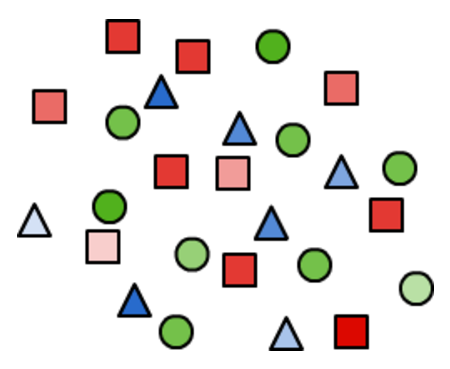
\includegraphics[scale=0.8]{figuras/ungroup-elements.eps}
    \label{fig:ungroup-elements}
    \caption{Elementos não agrupados}
  \end{subfigure}%
  \begin{subfigure}{.5\textwidth}
    \centering
    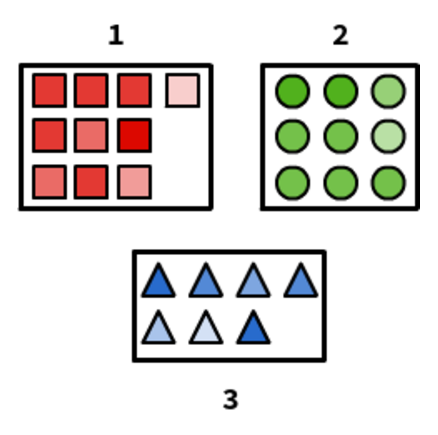
\includegraphics[scale=0.8]{figuras/group-elements.eps}
    \label{fig:group-elements}
    \caption{Elementos agrupados}
  \end{subfigure}
  \caption{Exemplo de clusterização}
\end{figure}

A clusterização é uma técnica da mineração de dados que consiste, justamente, em realizar o procedimento descrito acima: organizar um conjunto de elementos, usualmente representados por vetores ou pontos em um espaço multidimensional, em \textit{clusters} (ou agrupamentos), de acordo com alguma medida de similaridade. Ela representa uma das principais etapas da análise de dados, denominada análise de \textit{clusters} \cite{jain1999}.

Não existe uma técnica de clusterização universal capaz de revelar toda a variedade de estruturas que podem estar presentes em conjuntos de dados multidimensionais. Diferentes algoritmos dependem implicitamente de certas hipóteses a respeito da forma dos clusters, da definição da medida de similaridade e dos critérios de agrupamento \cite{estivill2002}.

\paragraph{Algorítmo \textit{k-means}}
\label{sub:k_means}

O algorítmo de clusterização \textit{k-means}, proposto por \citeonline{lloyd1957}, tem o objetivo de dividir \(N\) elementos em \(k\) grupos, onde cada elemento pertence ao \textit{cluster} mais próximo. O valor de \(k\) deve ser informado a priori, sendo menor que a quantidade de elementos.

Os passos do algoritmo são:

\begin{enumerate}
  \item \textbf{Gerar centróides:} neste passo os \(k\) centróides recebem valores iniciais. O valor inicial dos centróides podem ser definidos randomicamente, através de uma Gaussiana (com média e variância estimados a partir do conjunto de elementos) ou escolhendo aleatoriamente \(k\) dos \(N\) elementos como centróides iniciais ou definindo-os como centróides de \(k\) grupos escolhidos aleatoriamente a partir dos dados iniciais.
  \begin{figure}[h]
    \centering
    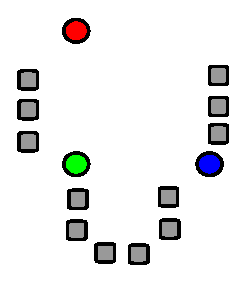
\includegraphics[scale=0.6]{figuras/kmeans-1.eps}
    \caption{k centróides (coloridos) recebem valores iniciais.}
  \end{figure}
  \item \textbf{Calcular distâncias:} aqui são calculadas as distâncias entre cada ponto e cada centróide. É a parte com maior peso computacional do algorítmo, já que o calculo é realizado para cada ponto.
  \item \textbf{Classificar os pontos:} cada ponto deve ser classificado de acordo com a distância entre ele e o centróide de cada \textit{cluster}. O ponto pertencerá ao \textit{cluster} cujo centróide está mais próximo. O algorítmo converge quando, em uma iteração, nenhum ponto mudar de \textit{cluster}.
  \begin{figure}[h]
    \centering
    \includegraphics[scale=0.6]{figuras/kmeans-2.eps}
    \caption{Cálculo das distâncias entre os pontos e os centróides.}
  \end{figure}
  \item \textbf{Calcular novos centróides:} para cada \textit{cluster}, um novo centróide é definido como a média desses pontos.
  \begin{figure}[h]
    \centering
    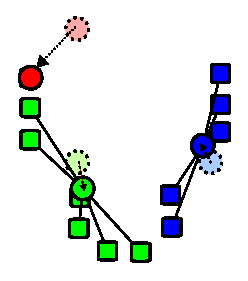
\includegraphics[scale=0.6]{figuras/kmeans-3.eps}
    \caption{Novos centróides definidos pela media dos elementos do \textit{cluster}.}
  \end{figure}
  \item \textbf{Repetir até convergir:} retorna ao passo 2. Como o resultado do algoritmo depende da escolha dos centróides iniciais, a convergência não é garantida ou ele converge para uma solução sub-ótima. Por isso, normalmente o algoritmo é executado várias vezes.
  \begin{figure}[h]
    \centering
    \includegraphics[scale=0.6]{figuras/kmeans-4.eps}
    \caption{O algorítmo converge quando nenhum ponto muda de \textit{cluster}.}
  \end{figure}
\end{enumerate}

Mudanças de escala ou de unidade de medidas para determinadas coordenadas dos elementos podem afetar a análise \cite{cole1998}. Sugere-se, então, que seja feito o processo de normalização (\textit{whitening}) dos dados antes da clusterização. A normalização consiste em ajustar a escala das distâncias de forma que os valores fiquem em intervalos padronizados, normalmente com média nula e variância 1.


\paragraph{Distância entre os pontos}
\label{ssub:distância_entre_os_pontos}

Segundo \citeonline{cole1998}, para clusterizar termos de acordo com sua similaridade, deve-se definir uma medida de quão próximos dois termos estão. Uma medida de distância (métrica) deve ser definida de tal forma que:

\begin{itemize}
  \item Seja sempre positiva.
  \item Seja simétrica: a distância de um termo \(A_{i}\) para um termo \(A_{j}\) deve ser a mesma de \(A_{j}\) para \(A_{i}\).
  \item Seja reflexiva: se a distância entre \(A_{i}\) e \(A_{j}\) é zero, então \(A_{i} = A_{j}\).
  \item Respeite a desigualdade triangular: considerando os termos (\(A_{i}, A_{j}\) e \(A_k\)), a distância \(d(A_{i}, A_k)\) deve ser menor ou igual à soma das distâncias \(d(A_{i}, A_{j})\) e \(d(A_{j}, A_k)\)
\end{itemize}

Existem várias medidas de distância. Começamos pela distância euclidiana entre dois pontos, \(A=(a_1, a_2, a_3, \ldots, a_n) \) e \(B=(b_1, b_2, b_3, \ldots, b_n) \), dada pela equação
%
\begin{align}
  dist(A, B) &= \sqrt{(a_1-b_1)^2+(a_2-b_2)^2+(a_3-b_3)^2+\ldots+(a_n-b_n)^2} \\
  dist(A, B) &= \sqrt{\displaystyle\sum_{i=1}^{n} (a_i-b_i)^2} \label{eq:euclidean}
\end{align}

Já a distância de Manhattan entre dois pontos, \(A=(a_1, a_2, a_3, \ldots, a_n) \) e \(B=(b_1, b_2, b_3, \ldots, b_n) \), é dada pela soma das diferenças absolutas de suas coordenadas:

\begin{align}
  dist(A, B) &= |a_1-b_1|+|a_2-b_2|+|a_3-b_3|+\ldots+|a_n-b_n| \\
  dist(A, B) &= \displaystyle\sum_{i=1}^{n} |a_i-b_i| \label{eq:manhattan}
\end{align}

Em ambos os casos, temos que a distância entre do ponto A ao ponto B é a mesma distância do ponto B ao ponto A.

\begin{figure}[h]
  \centering
  \begin{subfigure}{.5\textwidth}
    \centering
    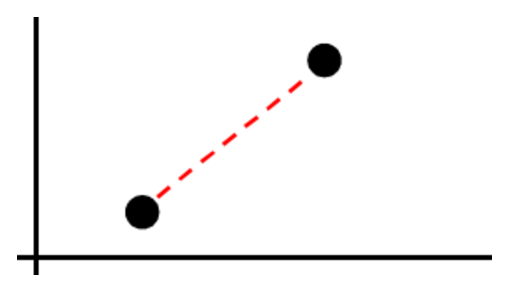
\includegraphics[scale=0.5]{figuras/euclidean.eps}
    \caption{Distância Euclidiana}
  \end{subfigure}%
  \begin{subfigure}{.5\textwidth}
    \centering
    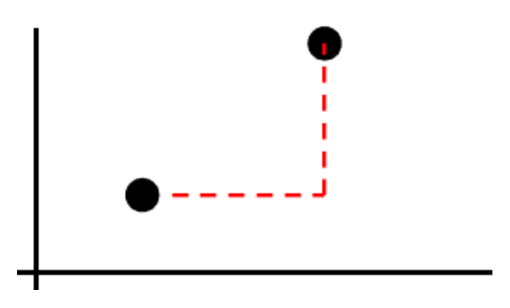
\includegraphics[scale=0.5]{figuras/manhattan.eps}
    \caption{Distância de Manhattan}
  \end{subfigure}
  \caption{Comparação entre distância euclidiana e de manhattan}
\end{figure}

Cada métrica pode gerar resultados diferentes no algoritmo \textit{k-means} e normalmente podem ser interpretadas do ponto de vista estatístico como uma escolha do modelo que gerou cada \textit{cluster}. A distância euclidiana pode ser associada a um modelo Gaussiano para gerar os pontos observados onde a média corresponde ao centróide de cada \textit{cluster} e o desvio padrão é o mesmo para todos os grupos.

\clearpage
\section{Aprendizado Semi-Supervisionado}

Essa forma de aprendizado é útil quando quando existem apenas alguns exemplos já classificados e pode ser utilizado tanto em tarefas de classificação quanto em tarefas de \textit{clustering}. A ideia do aprendizado semi-supervisionado é utilizar esses exemplos previamente classificados para se obter informações sobre o problema e utilizá-las para auxiliar o processo de aprendizado a partir de exemplos não classificados \cite{bruce}.

Existem várias estratégias para definir algoritmos de aprendizado semi-supervisionado. É comum utilizar modelos de aprendizado não-supervisionado com alterações, afim de se poder inserir informações a priori.

Podemos tornar o algoritmo \textit{k-means} semi-supervisionado se fixarmos \textit{clusters} específicos para determinados termos previamente classificados, de forma que esse eles sempre pertençam aos \textit{clusters} pré-fixados. Dessa forma, a informação inserida influenciará diretamente na posição dos \textit{clusters}.

No \textit{LDA}, também podemos fixar algumas linhas da tabela de mistura \(Q\). Dessa forma, podemos dizer que um texto pertence a um tópico específico ou a misturas específicas de tópicos.


\section{Distância entre os pontos}
\label{ssub:distância_entre_os_pontos}

Segundo \citeonline{cole1998}, para clusterizar termos de acordo com sua similaridade, deve-se definir uma medida de quão próximos dois termos estão. Uma medida de distância (métrica) deve ser definida de tal forma que:

\begin{itemize}
  \item Seja sempre positiva.
  \item Seja simétrica: a distância de um termo \(A_{i}\) para um termo \(A_{j}\) deve ser a mesma de \(A_{j}\) para \(A_{i}\).
  \item Seja reflexiva: se a distância entre \(A_{i}\) e \(A_{j}\) é zero, então \(A_{i} = A_{j}\).
  \item Respeite a desigualdade triangular: considerando os termos (\(A_{i}, A_{j}\) e \(A_k\)), a distância \(d(A_{i}, A_k)\) deve ser menor ou igual à soma das distâncias \(d(A_{i}, A_{j})\) e \(d(A_{j}, A_k)\)
\end{itemize}

Existem várias medidas de distância. Começamos pela distância Euclidiana entre dois pontos, \(A=(a_1, a_2, a_3, \ldots, a_n) \) e \(B=(b_1, b_2, b_3, \ldots, b_n) \), dada pela equação
%
\begin{align}
  dist(A, B) &= \sqrt{\displaystyle\sum_{i=1}^{n} (a_i-b_i)^2} \label{eq:euclidean}
\end{align}

Já a distância de Manhattan entre dois pontos, \(A=(a_1, a_2, a_3, \ldots, a_n) \) e \(B=(b_1, b_2, b_3, \ldots, b_n) \), é dada pela soma das diferenças absolutas de suas coordenadas:

\begin{align}
  dist(A, B) &= \displaystyle\sum_{i=1}^{n} |a_i-b_i| \label{eq:manhattan}
\end{align}

Em ambos os casos, temos que a distância entre do ponto A ao ponto B é a mesma distância do ponto B ao ponto A.

\begin{figure}[h]
  \centering
  \begin{subfigure}{.5\textwidth}
    \centering
    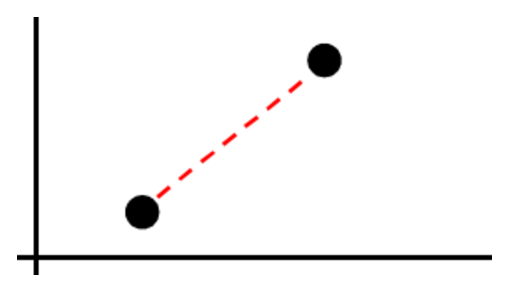
\includegraphics[scale=0.5]{figuras/euclidean.eps}
    \caption{Distância Euclidiana}
  \end{subfigure}%
  \begin{subfigure}{.5\textwidth}
    \centering
    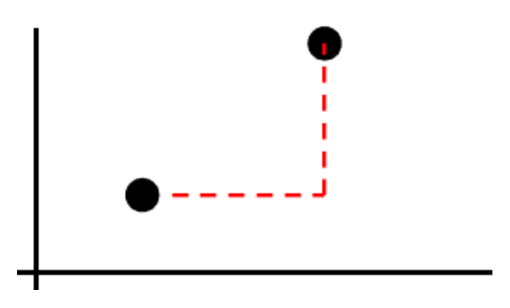
\includegraphics[scale=0.5]{figuras/manhattan.eps}
    \caption{Distância de Manhattan}
  \end{subfigure}
  \caption{Comparação entre distância Euclidiana e de Manhattan}
\end{figure}

Cada métrica pode gerar resultados diferentes no algoritmo \textit{k-means} e normalmente podem ser interpretadas do ponto de vista estatístico como uma escolha do modelo que gerou cada \textit{cluster}. A distância euclidiana pode ser associada a um modelo Gaussiano para gerar os pontos observados onde a média corresponde ao centróide de cada \textit{cluster} e o desvio padrão é o mesmo para todos os grupos.

\subsection{Validação Cruzada}

A validação cruzada é uma técnica geralmente utilizada para avaliar modelos preditivos, buscando estimar o quão preciso é o modelo avaliado. A ideia principal da validação cruzada consiste em dividir o conjunto de dados em subconjuntos mutualmente exclusivos, onde alguns desses subconjuntos serão utilizados para a estimação dos parâmetros do modelo (treinamento) e os outros subconjuntos serão utilizados para a validação do modelo (validação ou teste) \cite{kohavi1995}.

O método \textit{holdout} é uma forma de validação de cruzada comumente utilizada e consiste em dividir o conjunto de dados em dois subconjuntos mutualmente exclusivos, onde seus tamanhos podem, ou não, ser diferentes. Um subconjunto servirá para o treinamento do modelo e o outro para a sua validação. A proporção mais comum é considerar 2/3 dos dados para treinamento e 1/3 para a validação. Essa abordagem é indicada quando está disponível uma grande quantidade de dados, quando o conjunto de dados é muito pequeno, o erro calculado na predição pode sofrer muita variação \cite{kohavi1995}.

Uma das métricas mais simples para avaliar o modelo é a comparação item a item dos resultados esperados pelos resultados obtidos:
%
\begin{align}
P_{a}=\frac{N_{vp}}{N_{it}},
\end{align}
%
onde:

\begin{itemize}
    \item \(P_{a}\) é a porcentagem de acertos do modelo,
    \item \(N_{vp}\) é o número de itens classificados corretamente pelo modelo e
    \item \(N_{it}\) é o número total de itens que fazem parte do conjunto de testes.
\end{itemize}



\chapter{Metodologia}

Este capítulo aborda o planejamento e execução do projeto, contendo os procedimentos e técnicas utilizadas, possibilitando a sua  replicação. Tendo em vista os conceitos descritos nos capítulos anteriores, o presente trabalho tem como objetivo responder à seguinte questão problema:

\begin{center}
\textit{É possível extrair o perfil temático dos deputados através da análise dos seus discursos e proposições utilizando técnicas de aprendizado de máquina e processamento de linguagem natural?}
\end{center}

Além disso, será construído um \textit{website} com o intuito de fornecer uma forma melhor de visualização dos dados obtidos nesta análise, através de gráficos interativos que garantam que o usuário tenha uma boa experiência de usabilidade.

\section{Trabalhos Relacionados}

Durante a pesquisa bibliográfica realizada neste trabalho, encontrou-se alguns trabalhos que também fizeram análise de textos parlamentares utilizando aprendizado bayesiano. O Retórica Parlamentar\footnote{http://retorica.labhackercd.net/about.html}, idealizado por Davi Moreira\footnote{https://github.com/davi-moreira}, Manoel Galdino\footnote{https://github.com/mgaldino} e Luis Carli\footnote{https://github.com/luiscarli}, utiliza os discursos proferidos pelos parlamentares no Pequeno Expediente e no Grande Expediente da Câmara dos Deputados para promover a transparência do mandato e fornecer subsídios para o controle social com a divulgação dos temas mais debatidos em Plenário.

A técnica utilizada pelo Retórica para a classificação dos discursos é um modelo bayesiano hierárquico, descrito por \citeonline{grimmer2009}, onde através de aprendizado não supervisionado são gerados \(k\) \textit{clusters}, sendo \(k\) um valor escolhido ao executar o algoritmo. O resultado é exportado para o formato \textit{csv} e contém os termos mais frequentes de cada cluster. Em seguida, um especialista deve ler e rotular cada \textit{cluster}.

A visualização dos dados é feita através de um gráfico de bolhas, em que cada bolha representa a relevância (medida pela frequência) de cada tema dentre todos os deputados analisados. Dentro de cada bolha são colocados os deputados que enfatizam aquele tema nos seus discursos. Um deputado está associado a um único tema, que é o tema mais enfatizado por ele nos seus discursos.

\begin{figure}[h]
    \centering
    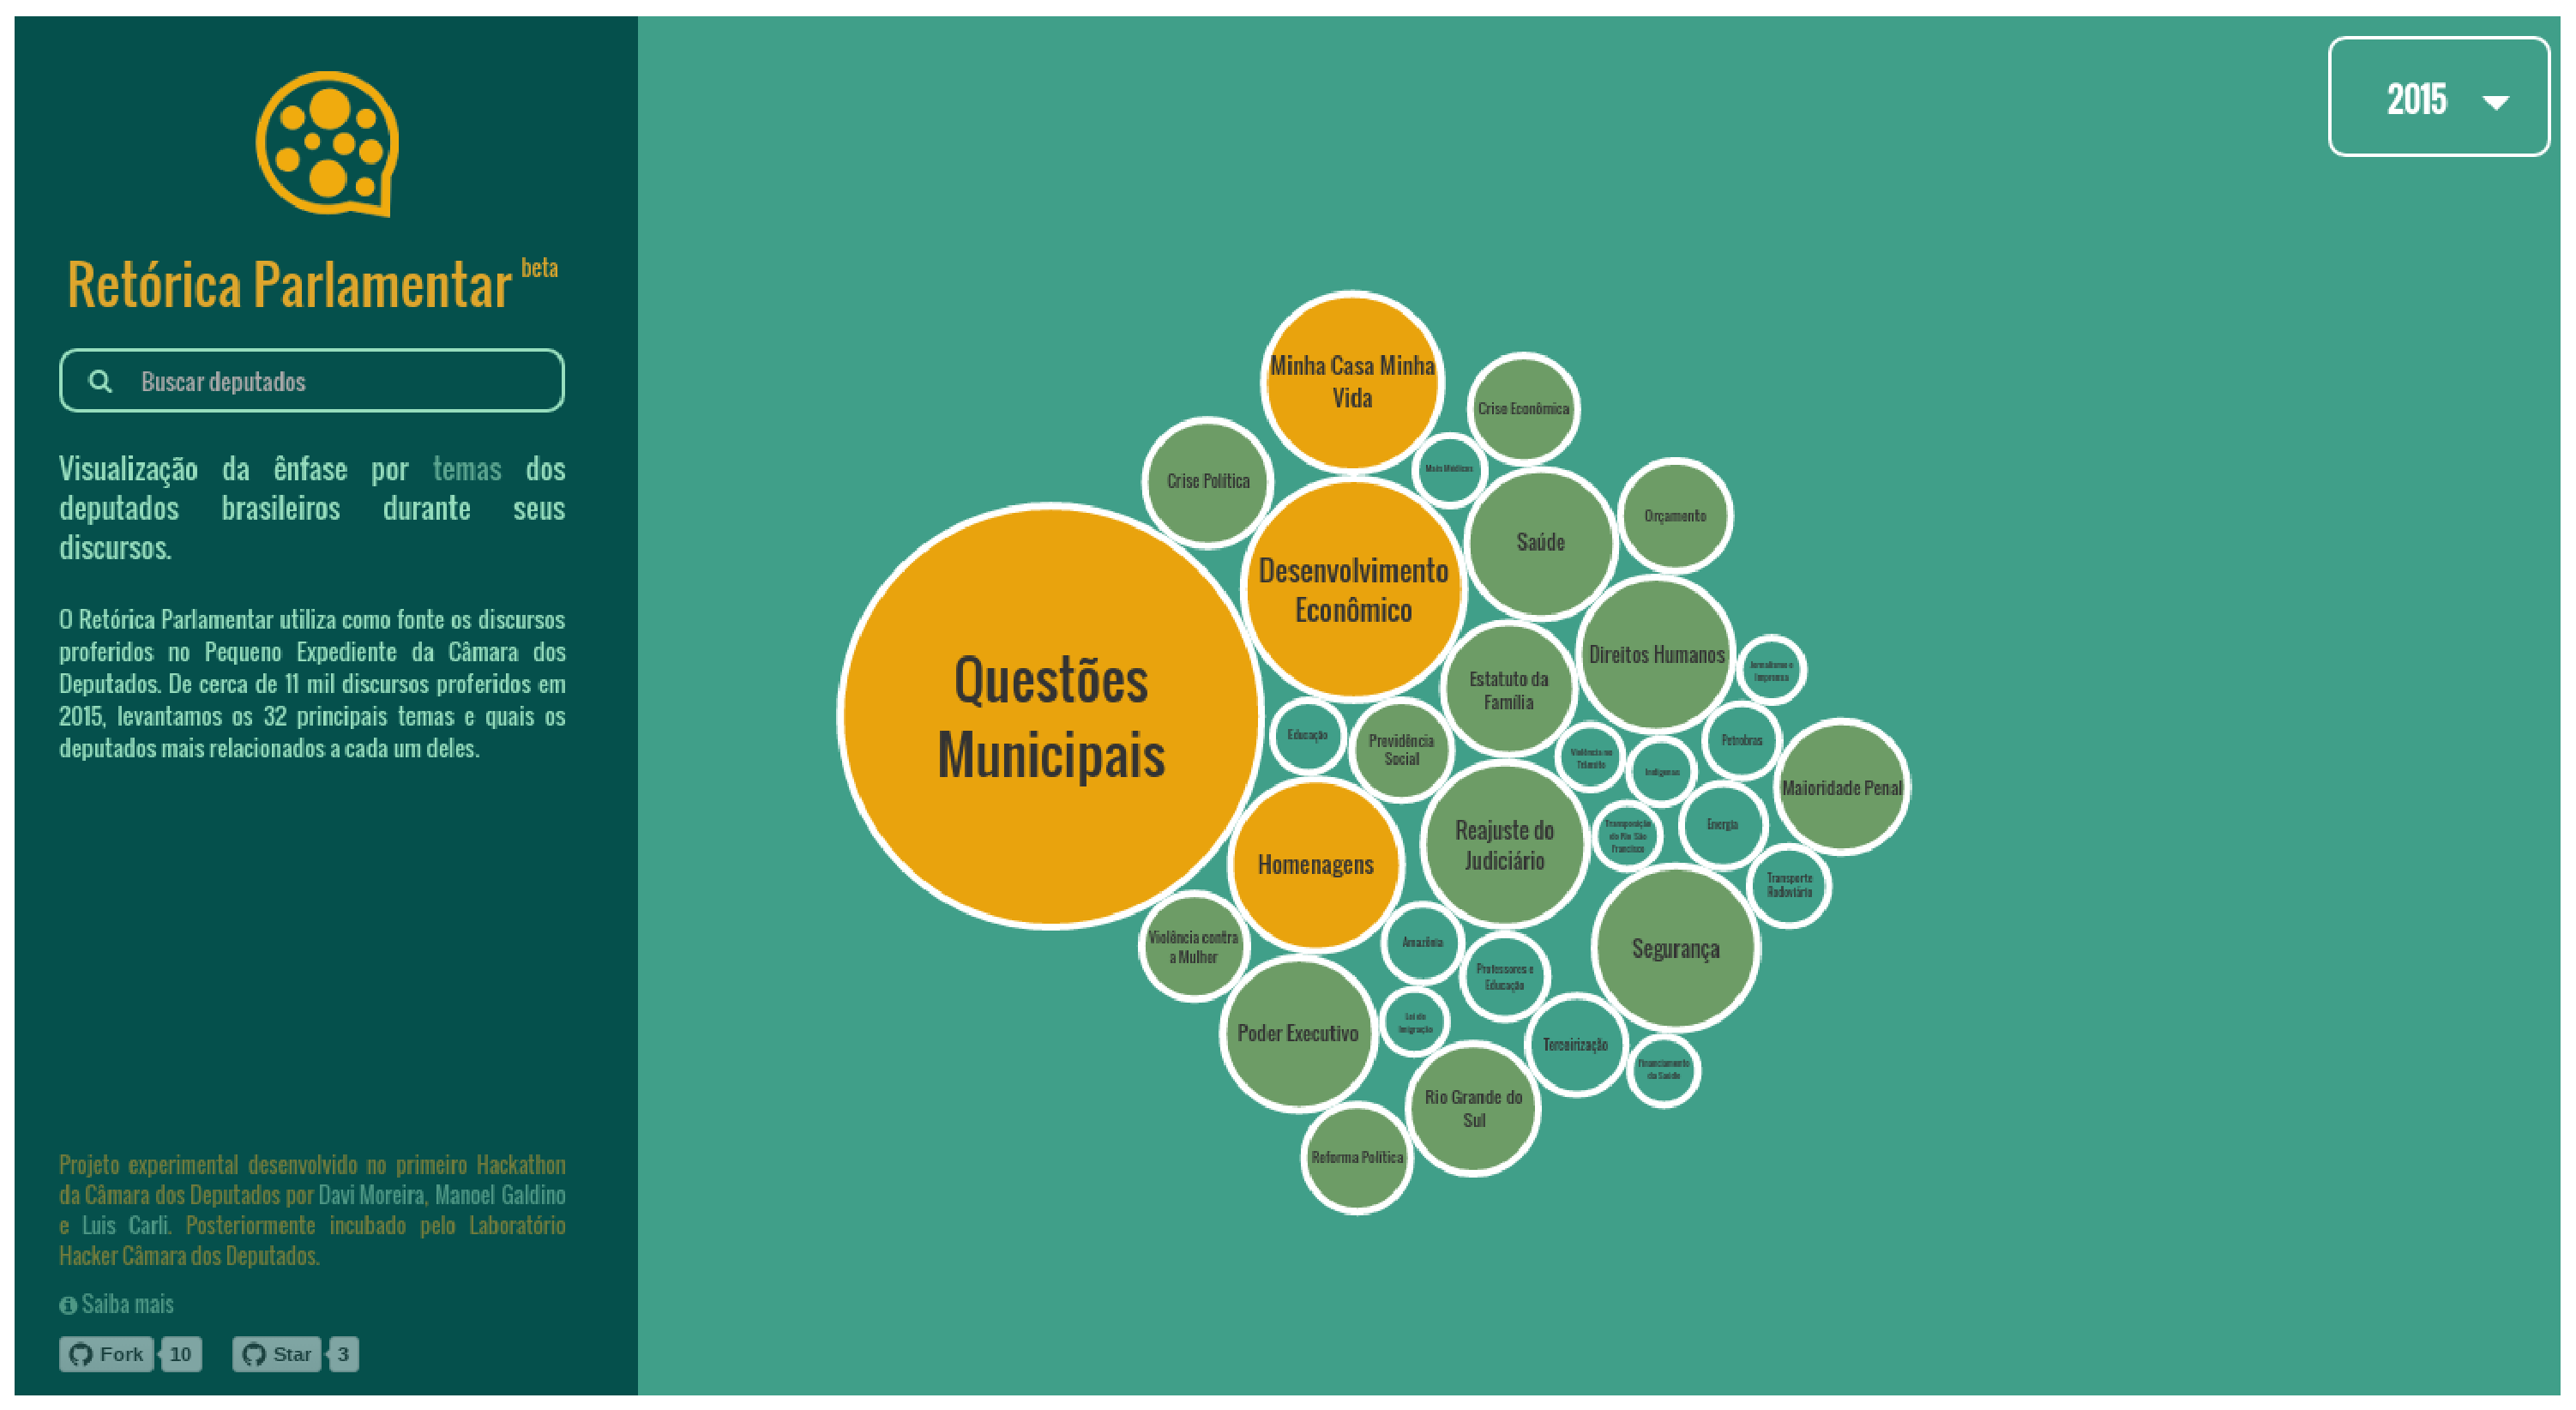
\includegraphics[scale=0.3]{figuras/retorica.eps}
    \caption{Retórica Parlamentar}
\end{figure}

\section{Planejamento das Atividades}

Para a realização desse trabalho, foram identificadas algumas atividades que seguem um fluxo de trabalho previsível, como mostra o diagrama a seguir:

As atividades realizadas

\begin{figure}[h]
    \centering
    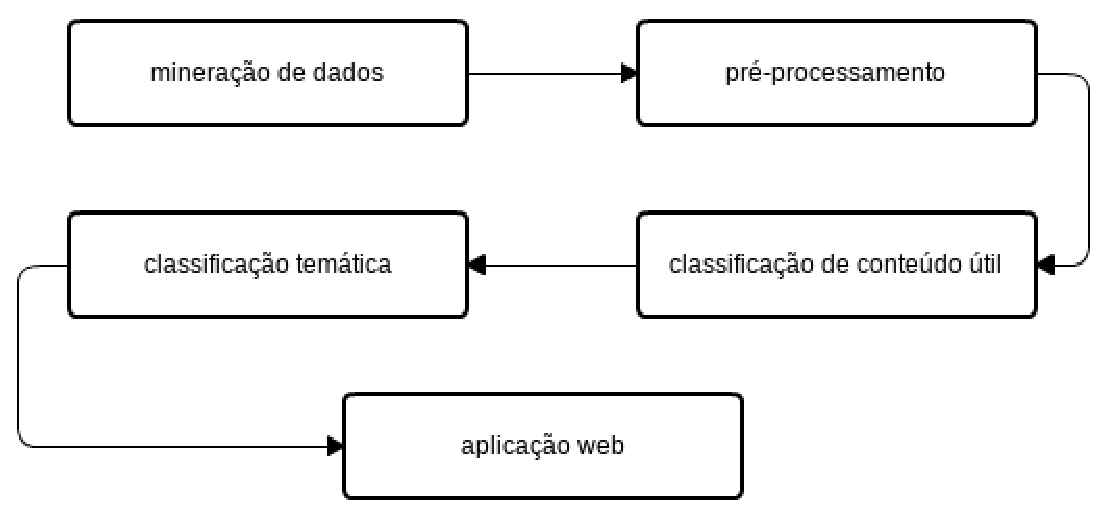
\includegraphics[scale=0.5]{figuras/planejamento.eps}
    \caption{Diagrama de planejamento}
\end{figure}

As seções seguintes descrevem cada etapa apresentada acima.

\subsection{Mineração de Dados}

A obtenção e persistência dos dados será realizada por uma biblioteca desenvolvida pelo autor, descrita na seção \ref{obtencao-dados} e consiste em realizar consultas ao \textit{webservice} da Câmara dos Deputados, fazendo um processamento inicial, afim de padronizar as informações e transformá-las em seus tipos correspondentes na linguagem \textit{Python}. Os dados provenientes do \textit{webservice} estão em formato \textit{XML} e armazenam valores como \textit{strings}.

Nesta etapa transformamos todos os campos com valores de números inteiros e decimais, datas, horários e textos em, respectivamente, valores \textit{Python} correspondentes. Além disso, também é realizada a persistência dessas informações em banco de dados relacional.

\subsection{Pré-processamento}

Apesar do ``pré-processamento'' não depender tanto dos dados reais, a definição das \textit{stop words} deve ser feita levando em consideração o conteúdo que será analisado.

A etapa de pré-processamento consiste na análise dos textos obtidos na mineração de dados, afim de identificar as \textit{stop words} presentes em textos do contexto legislativo. Além disso, deve ser realizada o processo de \textit{stemização} para reduzir a dimensionalidade das \textit{bag-of-words} geradas.

Estudamos diferentes estratégias para a utilização de \(n\)-gramas, mas por enquanto decidiu-se, por uma questão de simplicidade, limitar-se apenas ao uso de unigramas.

\subsection{Classificação Conteúdo Útil}

Essa classificação tem como objetivo melhorar a qualidade da análise temática dos deputados. Uma parte considerável dos textos não possuem valor semântico significativo, pois tratam de questões protocolares e de trâmite legislativo. Citamos um exemplo: \textit{``É preciso haver quórum de 257 Srs. Deputados para aprovação da matéria, quórum mínimo. A votação é normal. Então, acho que, quando houver uns 300 ou 320 votos, encerraremos.''}. Portanto, a classificação entre conteúdo útil/não-útil consiste em separar os parágrafos que realmente possuem valor para a análise posterior dos que não devem ser usados nestas análises.

Essa atividade não foi mais adotada para a segunda parte desse trabalho, pois optou-se pela não utilização dos textos completos dos discursos, substituindo-os pelos sumários e indexações. Com essa nova abordagem, a análise é feita utilizando um resumo (sumário) do discurso, onde cada frase, geralmente, representa um tema abordado pelo parlamentar. Também foi utilizado um conjunto de palavras que são utilizadas para a busca no próprio site da Câmara dos Deputados. Tanto os sumários quanto as indexação são elaborados por um departamento da Casa, por profissionais especializados em Arquitetura da Informação.

\subsection{Classificação Temática}

Após determinar quais parágrafos serão análisados, os mesmos devem ser classificados de acordo com alguns temas. Para o contexto do TCC 1, foram selecionados inicialmente: Agropecuária, Saúde, Esporte, Educação, Ciência e Tecnologia, Economia, Política, Meio Ambiente, Direitos Humanos e Segurança. Para a realização dessa tarefa, foi necessário construir um texto inicial para cada um dos temas listados, afim de fornecer um parâmetro inicial ao classificador. Os textos iniciais de cada tema têm como base textos previamente classificados em portais de notícias brasileiros e consistem em apenas uma listagem de palavras comuns relacionadas a estes temas.

Para o TCC 2, a base inicial de palavras foi obtida através do Tesauro da Câmara dos Deputados, que possui uma base de 14611 termos, agrupados em 49 áreas temáticas. Tal agrupamento foi realizado por profissionais da área de arquitetura da informação da própria Câmara.

54 temas é uma quantidade relativamente grande, o que poderia dificultar um pouco a análise. Foi realizado um agrupamento dessas áreas temáticas e reduzidos para 22 temas. As tabelas a seguir mostra todos os temas e seus agrupamentos (macro-temas):

\begin{table}[h]
\centering
\begin{tabular}{clc}
\hline
\multicolumn{1}{|c|}{\textbf{\begin{tabular}[c]{@{}c@{}}Quantidade\\ de Termos\end{tabular}}} & \multicolumn{1}{c|}{\textbf{Tema}} & \multicolumn{1}{c|}{\textbf{Macro-tema}} \\ \hline
\multicolumn{1}{|c|}{57} & \multicolumn{1}{l|}{Administração} & \multicolumn{1}{c|}{Gestão} \\ \hline
\rowcolor[HTML]{EFEFEF}
\multicolumn{1}{|c|}{\cellcolor[HTML]{EFEFEF}1481} & \multicolumn{1}{l|}{\cellcolor[HTML]{EFEFEF}Administração Pública} & \multicolumn{1}{c|}{\cellcolor[HTML]{EFEFEF}Administração Pública} \\ \hline
\multicolumn{1}{|c|}{304} & \multicolumn{1}{l|}{Agricultura, Pecuária e Pesca} & \multicolumn{1}{c|}{} \\ \cline{1-2}
\multicolumn{1}{|c|}{78} & \multicolumn{1}{l|}{Política Fundiária} & \multicolumn{1}{c|}{\multirow{-2}{*}{Agricultura, Pecuária e Pesca}} \\ \hline
\rowcolor[HTML]{EFEFEF}
\multicolumn{1}{|c|}{\cellcolor[HTML]{EFEFEF}{\color[HTML]{000000} 97}} & \multicolumn{1}{l|}{\cellcolor[HTML]{EFEFEF}{\color[HTML]{000000} Ciência da Informação}} & \multicolumn{1}{c|}{\cellcolor[HTML]{EFEFEF}} \\ \cline{1-2}
\rowcolor[HTML]{EFEFEF}
\multicolumn{1}{|c|}{\cellcolor[HTML]{EFEFEF}{\color[HTML]{000000} 221}} & \multicolumn{1}{l|}{\cellcolor[HTML]{EFEFEF}{\color[HTML]{000000} Arte e Cultura}} & \multicolumn{1}{c|}{\cellcolor[HTML]{EFEFEF}} \\ \cline{1-2}
\rowcolor[HTML]{EFEFEF}
\multicolumn{1}{|c|}{\cellcolor[HTML]{EFEFEF}{\color[HTML]{000000} 17}} & \multicolumn{1}{l|}{\cellcolor[HTML]{EFEFEF}{\color[HTML]{000000} Artes e Letras}} & \multicolumn{1}{c|}{\multirow{-3}{*}{\cellcolor[HTML]{EFEFEF}Artes, Cultura e Informação}} \\ \hline
\multicolumn{1}{|c|}{180} & \multicolumn{1}{l|}{Ciência e Tecnologia} & \multicolumn{1}{c|}{} \\ \cline{1-2}
\multicolumn{1}{|c|}{192} & \multicolumn{1}{l|}{Informática e TI} & \multicolumn{1}{c|}{} \\ \cline{1-2}
\multicolumn{1}{|c|}{264} & \multicolumn{1}{l|}{Comunicações} & \multicolumn{1}{c|}{\multirow{-3}{*}{Ciência e Tecnologia}} \\ \hline
\rowcolor[HTML]{EFEFEF}
\multicolumn{1}{|c|}{\cellcolor[HTML]{EFEFEF}45} & \multicolumn{1}{l|}{\cellcolor[HTML]{EFEFEF}Comércio Exterior} & \multicolumn{1}{c|}{\cellcolor[HTML]{EFEFEF}} \\ \cline{1-2}
\rowcolor[HTML]{EFEFEF}
\multicolumn{1}{|c|}{\cellcolor[HTML]{EFEFEF}132} & \multicolumn{1}{l|}{\cellcolor[HTML]{EFEFEF}Relações Internacionais} & \multicolumn{1}{c|}{\multirow{-2}{*}{\cellcolor[HTML]{EFEFEF}Relações Exteriores}} \\ \hline
\multicolumn{1}{|c|}{36} & \multicolumn{1}{l|}{Comunicação Social} & \multicolumn{1}{c|}{Comunicação Social} \\ \hline
\rowcolor[HTML]{EFEFEF}
\multicolumn{1}{|c|}{\cellcolor[HTML]{EFEFEF}139} & \multicolumn{1}{l|}{\cellcolor[HTML]{EFEFEF}Economia} & \multicolumn{1}{c|}{\cellcolor[HTML]{EFEFEF}} \\ \cline{1-2}
\rowcolor[HTML]{EFEFEF}
\multicolumn{1}{|c|}{\cellcolor[HTML]{EFEFEF}45} & \multicolumn{1}{l|}{\cellcolor[HTML]{EFEFEF}Contabilidade} & \multicolumn{1}{c|}{\cellcolor[HTML]{EFEFEF}} \\ \cline{1-2}
\rowcolor[HTML]{EFEFEF}
\multicolumn{1}{|c|}{\cellcolor[HTML]{EFEFEF}281} & \multicolumn{1}{l|}{\cellcolor[HTML]{EFEFEF}Finanças Públicas e Orçamento} & \multicolumn{1}{c|}{\cellcolor[HTML]{EFEFEF}} \\ \cline{1-2}
\rowcolor[HTML]{EFEFEF}
\multicolumn{1}{|c|}{\cellcolor[HTML]{EFEFEF}38} & \multicolumn{1}{l|}{\cellcolor[HTML]{EFEFEF}Política Econômica} & \multicolumn{1}{c|}{\cellcolor[HTML]{EFEFEF}} \\ \cline{1-2}
\rowcolor[HTML]{EFEFEF}
\multicolumn{1}{|c|}{\cellcolor[HTML]{EFEFEF}282} & \multicolumn{1}{l|}{\cellcolor[HTML]{EFEFEF}Sistema Financeiro} & \multicolumn{1}{c|}{\cellcolor[HTML]{EFEFEF}} \\ \cline{1-2}
\rowcolor[HTML]{EFEFEF}
\multicolumn{1}{|c|}{\cellcolor[HTML]{EFEFEF}235} & \multicolumn{1}{l|}{\cellcolor[HTML]{EFEFEF}Tributação} & \multicolumn{1}{c|}{\multirow{-6}{*}{\cellcolor[HTML]{EFEFEF}Economia e Finanças Públicas}} \\ \hline
\multicolumn{1}{|c|}{27} & \multicolumn{1}{l|}{Desenvolvimento Regional} & \multicolumn{1}{c|}{Desenvolvimento Regional} \\ \hline
\rowcolor[HTML]{EFEFEF}
\multicolumn{1}{|c|}{\cellcolor[HTML]{EFEFEF}61} & \multicolumn{1}{l|}{\cellcolor[HTML]{EFEFEF}Arquitetura e Urbanismo} & \multicolumn{1}{c|}{\cellcolor[HTML]{EFEFEF}} \\ \cline{1-2}
\rowcolor[HTML]{EFEFEF}
\multicolumn{1}{|c|}{\cellcolor[HTML]{EFEFEF}166} & \multicolumn{1}{l|}{\cellcolor[HTML]{EFEFEF}Desenvolvimento Urbano} & \multicolumn{1}{c|}{\multirow{-2}{*}{\cellcolor[HTML]{EFEFEF}Cidades}} \\ \hline
\multicolumn{1}{|c|}{285} & \multicolumn{1}{l|}{Desporto e Lazer} & \multicolumn{1}{c|}{} \\ \cline{1-2}
\multicolumn{1}{|c|}{125} & \multicolumn{1}{l|}{Turismo} & \multicolumn{1}{c|}{\multirow{-2}{*}{Esporte e Lazer}} \\ \hline
\rowcolor[HTML]{EFEFEF}
\multicolumn{1}{|c|}{\cellcolor[HTML]{EFEFEF}1033} & \multicolumn{1}{l|}{\cellcolor[HTML]{EFEFEF}Direito Civil e Processual Civil} & \multicolumn{1}{c|}{\cellcolor[HTML]{EFEFEF}} \\ \cline{1-2}
\rowcolor[HTML]{EFEFEF}
\multicolumn{1}{|c|}{\cellcolor[HTML]{EFEFEF}134} & \multicolumn{1}{l|}{\cellcolor[HTML]{EFEFEF}Direito e Justiça} & \multicolumn{1}{c|}{\multirow{-2}{*}{\cellcolor[HTML]{EFEFEF}Justica}} \\ \hline
\multicolumn{1}{|c|}{1756} & \multicolumn{1}{l|}{Direito Constitucional} & \multicolumn{1}{c|}{Direito Constitucional} \\ \hline
\rowcolor[HTML]{EFEFEF}
\multicolumn{1}{|c|}{\cellcolor[HTML]{EFEFEF}115} & \multicolumn{1}{l|}{\cellcolor[HTML]{EFEFEF}Direito e Defesa do Consumidor} & \multicolumn{1}{c|}{\cellcolor[HTML]{EFEFEF}} \\ \cline{1-2}
\rowcolor[HTML]{EFEFEF}
\multicolumn{1}{|c|}{\cellcolor[HTML]{EFEFEF}477} & \multicolumn{1}{l|}{\cellcolor[HTML]{EFEFEF}Indústria e Comércio} & \multicolumn{1}{c|}{\multirow{-2}{*}{\cellcolor[HTML]{EFEFEF}Comércio e Consumidor}} \\ \hline
\end{tabular}
\caption{Relação de Temas - Tesauro da Câmara dos Deputados (Parte I)}
\end{table}

\clearpage

\begin{table}[h]
\centering
\begin{tabular}{clc}
\hline
\multicolumn{1}{|c|}{\textbf{\begin{tabular}[c]{@{}c@{}}Quantidade\\ de Termos\end{tabular}}} & \multicolumn{1}{c|}{\textbf{Tema}} & \multicolumn{1}{c|}{\textbf{Macro-tema}} \\ \hline
\multicolumn{1}{|c|}{150} & \multicolumn{1}{l|}{Defesa e Segurança Nacional} & \multicolumn{1}{c|}{} \\ \cline{1-2}
\multicolumn{1}{|c|}{874} & \multicolumn{1}{l|}{Direito Penal} & \multicolumn{1}{c|}{} \\ \cline{1-2}
\multicolumn{1}{|c|}{264} & \multicolumn{1}{l|}{Segurança Pública} & \multicolumn{1}{c|}{\multirow{-3}{*}{Segurança}} \\ \hline
\rowcolor[HTML]{EFEFEF}
\multicolumn{1}{|c|}{\cellcolor[HTML]{EFEFEF}1054} & \multicolumn{1}{l|}{\cellcolor[HTML]{EFEFEF}Direito do Trabalho} & \multicolumn{1}{c|}{\cellcolor[HTML]{EFEFEF}} \\ \cline{1-2}
\rowcolor[HTML]{EFEFEF}
\multicolumn{1}{|c|}{\cellcolor[HTML]{EFEFEF}210} & \multicolumn{1}{l|}{\cellcolor[HTML]{EFEFEF}Trabalho e Emprego} & \multicolumn{1}{c|}{\multirow{-2}{*}{\cellcolor[HTML]{EFEFEF}Trabalho}} \\ \hline
\multicolumn{1}{|c|}{667} & \multicolumn{1}{l|}{Educação} & \multicolumn{1}{c|}{Educação} \\ \hline
\rowcolor[HTML]{EFEFEF}
\multicolumn{1}{|c|}{\cellcolor[HTML]{EFEFEF}318} & \multicolumn{1}{l|}{\cellcolor[HTML]{EFEFEF}\begin{tabular}[c]{@{}l@{}}Meio Ambiente e Desenvolvimento\\ Sustentável\end{tabular}} & \multicolumn{1}{c|}{\cellcolor[HTML]{EFEFEF}} \\ \cline{1-2}
\rowcolor[HTML]{EFEFEF}
\multicolumn{1}{|c|}{\cellcolor[HTML]{EFEFEF}263} & \multicolumn{1}{l|}{\cellcolor[HTML]{EFEFEF}\begin{tabular}[c]{@{}l@{}}Recursos Hídricos, Minerais e\\ Política Energética\end{tabular}} & \multicolumn{1}{c|}{\multirow{-2}{*}{\cellcolor[HTML]{EFEFEF}Meio Ambiente e Energia}} \\ \hline
\multicolumn{1}{|c|}{19} & \multicolumn{1}{l|}{Ciência Política} & \multicolumn{1}{c|}{} \\ \cline{1-2}
\multicolumn{1}{|c|}{1610} & \multicolumn{1}{l|}{Processo Legislativo} & \multicolumn{1}{c|}{} \\ \cline{1-2}
\multicolumn{1}{|c|}{552} & \multicolumn{1}{l|}{Organização Política} & \multicolumn{1}{c|}{\multirow{-3}{*}{Política}} \\ \hline
\rowcolor[HTML]{EFEFEF}
\multicolumn{1}{|c|}{\cellcolor[HTML]{EFEFEF}208} & \multicolumn{1}{l|}{\cellcolor[HTML]{EFEFEF}Direitos Humanos e Minorias} & \multicolumn{1}{c|}{\cellcolor[HTML]{EFEFEF}} \\ \cline{1-2}
\rowcolor[HTML]{EFEFEF}
\multicolumn{1}{|c|}{\cellcolor[HTML]{EFEFEF}21} & \multicolumn{1}{l|}{\cellcolor[HTML]{EFEFEF}Antropologia} & \multicolumn{1}{c|}{\cellcolor[HTML]{EFEFEF}} \\ \cline{1-2}
\rowcolor[HTML]{EFEFEF}
\multicolumn{1}{|c|}{\cellcolor[HTML]{EFEFEF}45} & \multicolumn{1}{l|}{\cellcolor[HTML]{EFEFEF}Teologia} & \multicolumn{1}{c|}{\cellcolor[HTML]{EFEFEF}} \\ \cline{1-2}
\rowcolor[HTML]{EFEFEF}
\multicolumn{1}{|c|}{\cellcolor[HTML]{EFEFEF}9} & \multicolumn{1}{l|}{\cellcolor[HTML]{EFEFEF}Demografia} & \multicolumn{1}{c|}{\multirow{-4}{*}{\cellcolor[HTML]{EFEFEF}Direitos Humanos e Minorias}} \\ \hline
\multicolumn{1}{|c|}{120} & \multicolumn{1}{l|}{Previdência e Assistência Social} & \multicolumn{1}{c|}{} \\ \cline{1-2}
\multicolumn{1}{|c|}{25} & \multicolumn{1}{l|}{Serviço Social} & \multicolumn{1}{c|}{} \\ \cline{1-2}
\multicolumn{1}{|c|}{87} & \multicolumn{1}{l|}{Sociologia} & \multicolumn{1}{c|}{\multirow{-3}{*}{Assistência Social}} \\ \hline
\rowcolor[HTML]{EFEFEF}
\multicolumn{1}{|c|}{\cellcolor[HTML]{EFEFEF}938} & \multicolumn{1}{l|}{\cellcolor[HTML]{EFEFEF}Saúde} & \multicolumn{1}{c|}{\cellcolor[HTML]{EFEFEF}Saúde} \\ \hline
\multicolumn{1}{|c|}{660} & \multicolumn{1}{l|}{Viação e Transporte} & \multicolumn{1}{c|}{Viação e Transporte} \\ \hline
\end{tabular}
\caption{Relação de Temas - Tesauro da Câmara dos Deputados (Parte II)}
\end{table}

\subsection{Aplicação \textit{Web}}

Os dados obtidos da classificação temática serão utilizados para alimentar um sistema \textit{web} para a exibição dos
mesmos. As principais funcionalidades planejadas são: visualizar os temas mais abordados por deputados, organizados por região, partido e bancada, visualizar todos os temas de uma determinada categoria, bem como o quanto cada tema é discutido e visualizar todos os temas abordados por um determinado deputado, mostrando separadamente os temas abordados em seus discursos e nas suas proposições. Os protótipos das telas do sistema estão disponíveis no apêndice \ref{prototipos-apendice}.

A primeira versão do Tenho Dito está disponível sub o domínio do Laboratório Hacker da Câmara dos Deputados e conta com apenas uma das funcionalidades prevista nos protótipos no apêndice \ref{prototipos-apendice}. Após a entrega final desse trabalho, a ferramenta continuará sendo desenvolvida pela equipe de desenvolvedores do Laboratório Hacker, onde as outras funcionalidades previstas serão implementadas, bem como novas funcionalidades. Por enquanto, apenas a visualização por estados foi implementada.

\section{Ferramentas e Tecnologias}
\label{ferramentas}

\subsection{Linguagem de Programação}

Devido ao tamanho da comunidade, grande utilização na área de aprendizado de máquina, possibilidade de desenvolvimento \textit{web} e conhecimento prévio do autor e orientador, decidiu-se utilizar a linguagem \textit{Python}\footnote{\lnk{Python}{https://www.python.org}} para o desenvolvimento das aplicações do presente trabalho.

\subsection{\textit{Frameworks} e Bibliotecas}

O desenvolvimento da aplicação \textit{web}, utilizará o \textit{framework} \textit{Django}\footnote{\lnk{Framework Django}{https://www.djangoproject.com}}, o que implica no uso da arquitetura \textit{MVT} (\textit{Model View Template}). Similar ao \textit{MVC}, no \textit{MVT} o ciclo começa por uma ação do usuário, a View notifica a Model, para que seu estado seja atualizado, a Model efetua as modificações necessárias e alerta as suas dependências que foi alterada, assim a Template consulta o novo estado da Model, e atualiza a sua visualização.

Além disso, utilizou-se a biblioteca \textit{Javascript} D3.js\footnote{\lnk{Biblioteca D3.js}{https://d3js.org/}} para auxiliar na visualização de dados. Por possuir características que podem facilitar o desenvolvimento, como \textit{default parameters}, \textit{arrow functions} e Classes, o código \textit{Javascript} desse trabalho será escrito utilizando a versão \textit{ES6}\footnote{http://es6-features.org/} (ou \textit{ECMAScript 6}) e para garantir melhor suporte aos navegadores mais antigos, será utilizado também o \textit{Babel}\footnote{https://babeljs.io/}, um \textit{transpiler} que transforma o código \textit{ES 6} em código \textit{ES 5}, suportado pela maioria dos navegadores atuais. Os estilos serão todos escritos utilizando a sintaxe \textit{SCSS} e as ferramentas \textit{node-sass} e \textit{postcss} para transformar o código \textit{SCSS} em \textit{CSS}, além de adicionar estilos de suporte \textit{cross-browser} automaticamente.

Esse trabalho não está focado na implementação de algoritmos de processamento de linguagem natural e aprendizado de máquina, mas sim na integração de algoritmos implementados por bibliotecas de terceiros. Serão utilizadas as bibliotecas \textit{plagiarism}\footnote{\lnk{Plagiarism}{https://github.com/fabiommendes/plagiarism}}, \textit{gensim}\footnote{https://radimrehurek.com/gensim/} e \textit{texblob}\footnote{\lnk{Texblob}{https://textblob.readthedocs.io}}, que encapsula a biblioteca \textit{NLTK}\footnote{http://www.nltk.org}, para tarefas de processamento de linguagem natural e aprendizado de máquina. Alguns cálculos são implementados utilizando o \textit{stack} científico do \textit{Python}, que inclui o \textit{numpy}\footnote{\lnk{NumPy}{http://www.numpy.org}}, \textit{scipy}\footnote{https://www.scipy.org}, \textit{matplotlib}\footnote{http://matplotlib.org} e \textit{sklearn}\footnote{http://scikit-learn.org}.

\subsection{Gerenciador de Repositórios de Código}

O gerenciamento de versões dos códigos das aplicações desenvolvidas utiliza o \textit{Git}\footnote{https://git-scm.com} e o serviço de \textit{web hosting} compartilhado \textit{GitHub}\footnote{https://github.com}. Além disso, os pacotes \textit{Python} são enviados para o \textit{PyPI}\footnote{https://pypi.python.org/pypi}, sendo facilmente instaláveis por terceiros através do comando \textit{pip}\footnote{https://pip.pypa.io}.


\subsection{Gerenciamento de Tarefas}

O controle de tarefas executadas ou em execução é feito utilizando o sistema de \textit{issues} e quadro de projetos do \textit{GitHub}.




\chapter{Resultados Obtidos}

\section{Obtenção dos Dados}
\label{obtencao-dados}

Todos os dados utilizados para análise foram obtidos através do portal de dados abertos da Câmara dos Deputados\footnote{http://www.camara.leg.br/transparencia/dados-abertos}, que é dividido em duas partes: dados legislativos e dados referentes à cota parlamentar, que não foram utilizados nesse trabalho. Os dados legislativos estão relacionados à informações sobre deputados, órgãos legislativos, proposições, sessões plenárias e reuniões de comissões.

\subsection{\textit{Webservice} da Câmara dos Deputados}

Atualmente, o \textit{Webservice} da Câmara dos Deputados é estruturado de acordo com os padrões \textit{SOAP} (\textit{Simple Object Access Protocol}, em português Protocolo Simples de Acesso a Objetos), que se baseiam na linguagem de marcação \textit{XML} e utilizam, principalmente, chamada de procedimento remoto (\textit{RPC}) e protocolo de transferência de hipertexto (\textit{HTTP}) para a transmissão das mensagens \cite{soap2007}.


No entanto, o \textit{webservice} possui alguns aspectos que podem ser melhorados. Como os dados são fornecidos utilizando o formato \textit{XML}, eles não são ``tipados'', ou seja, independente do tipo (inteiro, data, texto, etc) eles são representados com \textit{strings}. Alguns dados são ambíguos, como os referentes aos deputados, onde existem ``ideCadastro'' e ``idParlamentar'', que são utilizados como parâmetros de entrada de requisições distintas. Outro problema é que requisições comuns precisam ser feitas indiretamente pois não agrega conteúdos com \textit{queries} relacionais, como normalmente são as \textit{API REST}. Além disso, o inteiro teor dos discursos parlamentares estão disponíveis apenas em formato \textit{RTF}, o que dificulta um pouco a utilização dos mesmos.

No momento de escrita desse trabalho, se encontra em desenvolvimento uma nova versão do portal de dados abertos da Câmara dos Deputados, que está em fase de testes e já pode ser acessada pela sociedade\footnote{https://dadosabertos.camara.leg.br/}, porém ainda não possui os mesmos dados disponíveis na versão anterior. O novo \textit{webservice} segue os padrões REST e possibilita a escolha do formato de retorno, podendo ser em \textit{XML} ou em  \textit{JSON}. Além disso, visa corrigir os problemas encontrados na versão anterior (alguns mencionados no parágrafo acima), bem como aumentar a quantidade de dados disponíveis. Uma das promessas é disponibilizar o texto completo das proposições, que hoje só é disponível via \textit{PDF} sendo que alguns são apenas imagens \textit{scaneadas} dos documentos físicos.

A estrutura do \textit{webservice} da Câmara dos Deputados pode ser encontrada no apêndice \ref{estrutura-webservice}

\section{Proposta de Desenvolvimento}

\subsection{\textit{Pygov-br}}

\textit{Pygov-br} é uma biblioteca \textit{python} desenvolvida no contexto desse trabalho cujo objetivo é centralizar o consumo de \textit{APIs} e \textit{webservices} governamentais brasileiros. Além dos dados, a biblioteca também irá fornecer um conjunto de \textit{plugins} para os principais \textit{frameworks} para desenvolvimento \textit{web}, para facilitar a utilização dos dados abertos, bem como o cruzamento de dados provenientes de diferentes órgãos governamentais.

Atualmente, a biblioteca oferece suporte somente ao \textit{webservice} da Câmara dos Deputados, tanto para o consumo dos dados quanto para o uso em aplicações \textit{Django}, já que para o desenvolvimento do presente trabalho apenas esses dados seriam utilizados.

A estrutura para o consumo dos \textit{webservices} não é fixa, pois cada \textit{webservice} possui suas características. A implementação para consumir os dados da Câmara dos Deputados segue a estrutura do \textit{webservice} (figura \ref{estrutua_camara_deputados}), com algumas alterações. Além disso, todos o código implementado foi escrito em inglês, apesar dos dados estarem em português.

\begin{figure}[h]
    \centering
    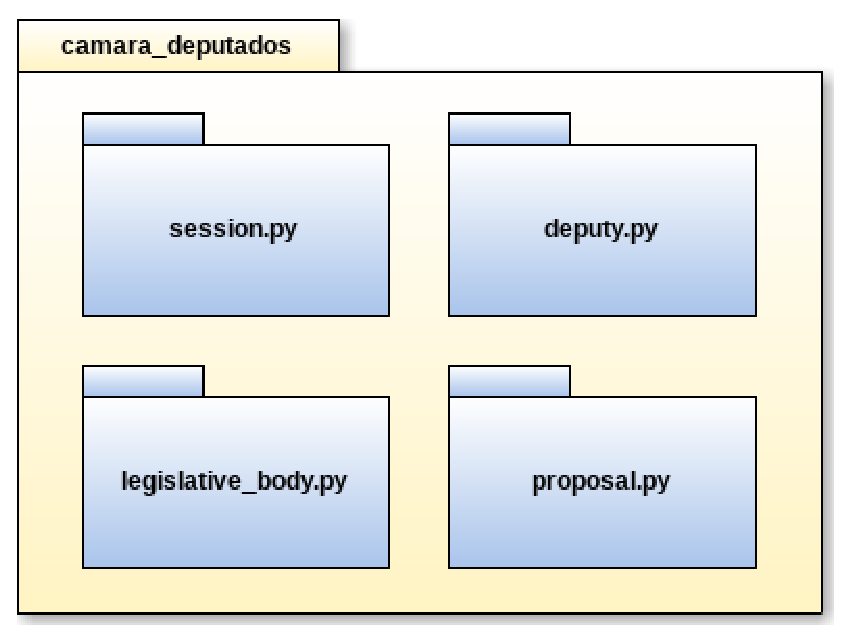
\includegraphics[scale=0.5]{figuras/camara_deputados.eps}
    \caption{Estrutura do módulo de consumo de dados da Câmara dos Deputados}
    \label{estrutua_camara_deputados}
\end{figure}


Como dito anteriormente, a \textit{pygov-br} também possui módulos para utilização em conjunto com os \textit{frameworks} de desenvolvimento \textit{web} mais utilizados na comunidade. Porém, como a solução \textit{web} desenvolvida nesse trabalho utilizará o \textit{framework Django}, a atual implementação da \textit{pygov-br} possui suporte somente a esse \textit{framework}.

O módulo \textbf{django\_apps} contém os \textit{plugins} para utilização em projetos \textit{Django}. Esses \textit{apps} possuem apenas as \textit{models} (na linguagem da arquitetura \textit{MVT} do \textit{Django}) já que o objetivo é somente facilitar a permanência das informações obtidas dos \textit{webservices} governamentais em um banco de dados. No caso da Câmara dos Deputados, os dados utilizados nesse trabalho ficam disponíveis seguindo o modelo entidade-relacionamento na figura \ref{modelo-eer}. Podemos notar que todas as colunas de todas as tabelas se encontram em em inglês, por motivos de padronização do código.

Após a apresentação da primeira parte desse trabalho, foram realizadas algumas sugestões quanto à tradução dos termos para o inglês. Entretanto, como estava prevista uma nova API da Câmara dos Deputados com alterações significativas que implicariam em uma reescrita considerável do código da \textit{pygov-br}, ficou decidido que essas alterações de nomenclaturas seriam realizadas no momento de reescrita da biblioteca.


\begin{figure}[h]
    \centering
    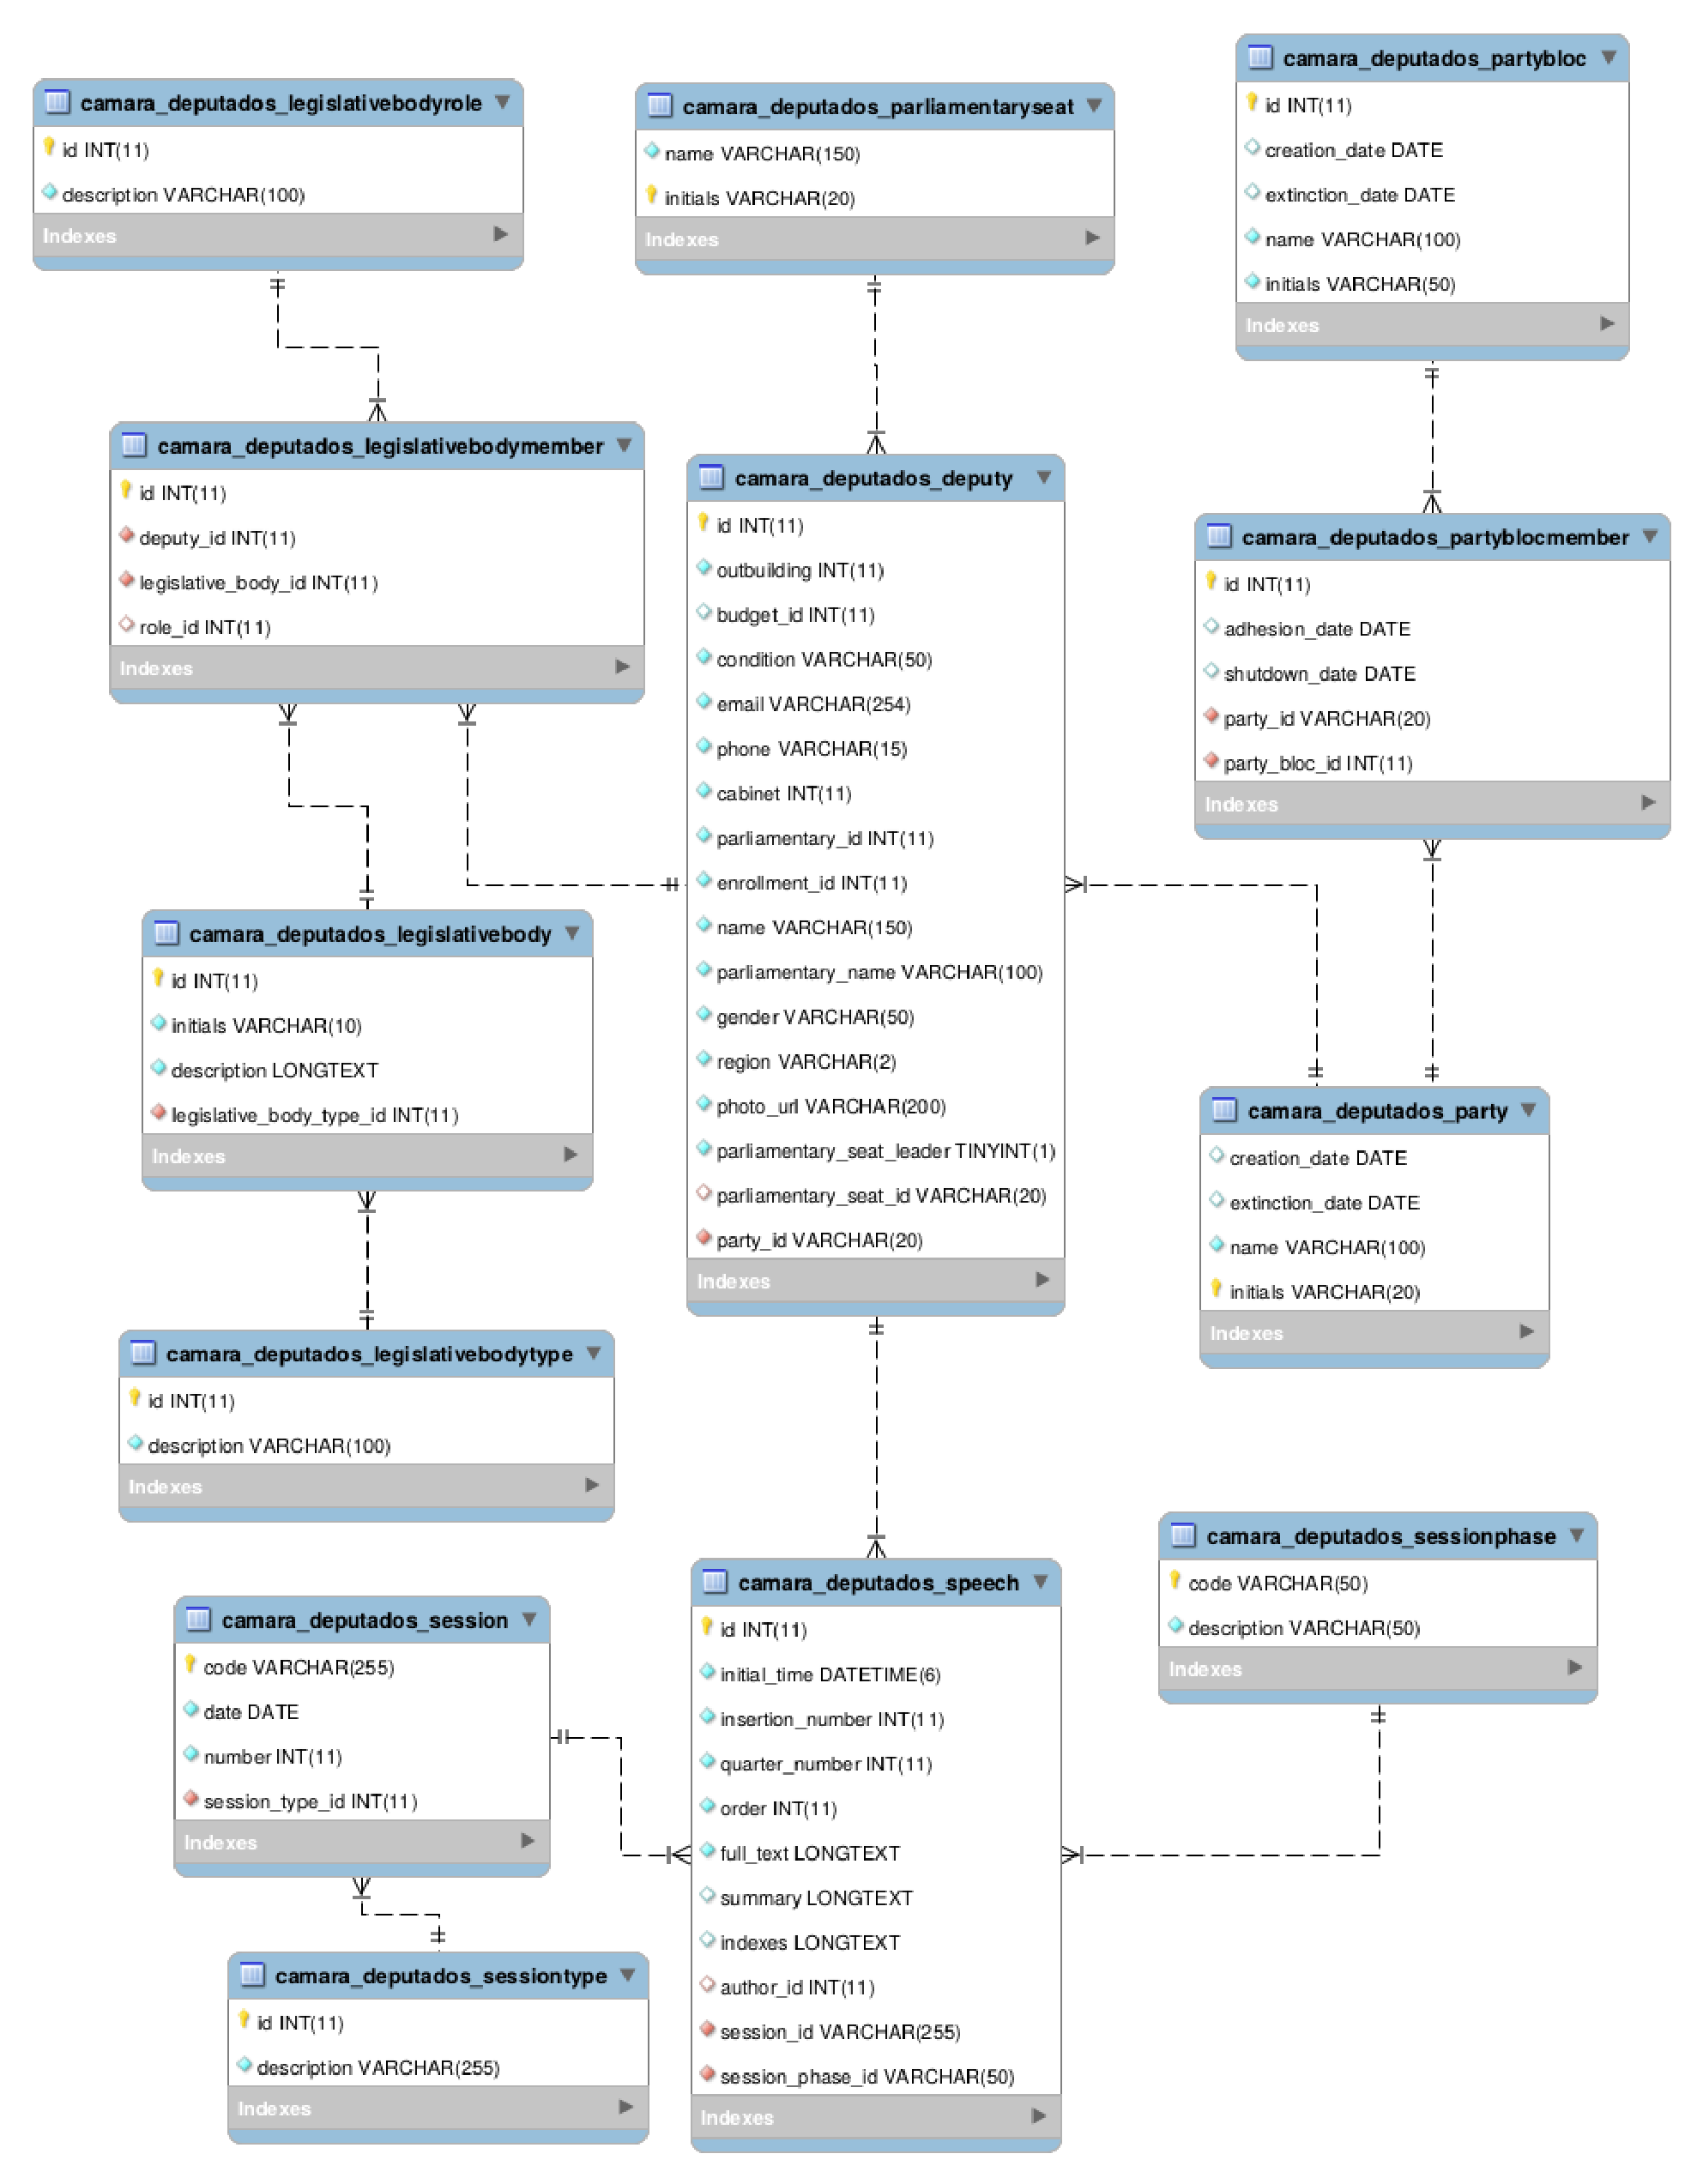
\includegraphics[scale=0.5]{figuras/pygov-eer.eps}
    \caption{Modelo entidade-relacionamento do banco de dados utilizado}
    \label{modelo-eer}
\end{figure}

\clearpage

\subsection{Tenho Dito}

``Tenho Dito'' é uma aplicação \textit{web}, desenvolvida utilizando a linguagem \textit{python} com o \textit{framework Django}, e tem como objetivo ser uma forma mais lúdica de visualização dos dados disponíveis nos \textit{webservices} de dados abertos da Câmara dos Deputados. Utiliza métodos de processamento de linguagem natural e aprendizado de máquina para extrair o perfil temático dos parlamentares, analisando o texto de seus discursos e proposições. Além disso, também é possível traçar os temas mais discutidos (tanto em propostas quanto nos próprios discursos) pelos deputados de uma determinada região ou por partidos.

A aplicação é divida em dois grandes módulos: \textit{nlp} e \textit{core}. O primeiro é responsável por todas as operações relacionadas ao processamento dos textos, o que inclui aprendizado de máquina. Já o segundo módulo é responsável pela parte \textit{web}. No momento de escrita desse trabalho, ainda não tinha sido implementado o segundo módulo. Entretanto, estão disponíveis alguns protótipos, que mostram as possíveis funcionalidades do sistema.

Conforme mencionado no item ``\textit{frameworks}'', em \ref{ferramentas}, a análise dos textos será realizada com o apoio das ferramentas:

\begin{itemize}
    \item \textbf{Plagiarism:} biblioteca desenvolvida pelo professor orientador do autor desse trabalho, Fábio Macêdo Mendes, e possui uma série de funcionalidades utilizadas no pré-processamento dos textos, como extração de \textit{tokens}, \textit{stemização}, remoção de \textit{stop words}, geração de \textit{n-gramas} e geração de \textit{bag-of-words} (com os diferentes tipos de representação dos termos, descrito na seção \ref{sec:representação_dos_termos} desse trabalho).
    \item \textbf{Textblob:} biblioteca \textit{python} para processamento de dados textuais. Ela fornece uma interface simples para realizar tarefas comuns do processamento de linguagem natural, como análise de sentimento e classificação, por exemplo. Utiliza a biblioteca \textit{LNTK} para realizar essas tarefas.
\end{itemize}

\subsubsection{Classificação dos Discursos}

A classificação dos discursos é dividida em duas etapas. A primeira etapa consiste em, inicialmente, dividir o texto em parágrafos, para que a análise seja realizada com uma quantidade menor de texto, e em seguida os parágrafos são classificados entre ``protocolo parlamentar'' ou ``conteúdo''. Por exemplo, o trecho ``É preciso haver quórum de 257 Srs. Deputados para aprovação da matéria, quórum mínimo. A votação é normal. Então, acho que, quando houver uns 300 ou 320 votos, encerraremos.'' não representa um conteúdo significativo, da mesma forma que ``O SR. ALCEU MOREIRA - Sr. Presidente, primeiro a medida provisória, logicamente.'' também não agregaria nenhum valor à análise. Trechos como esses devem se classificados como ``protocolo parlamentar'' e descartados da análise temática. A segunda etapa do processamento é a classificação temática dos parágrafos classificados como ``conteúdo'', na etapa anterior.

Para ambas etapas o procedimento adotado é o mesmo, com algumas alterações nos classificadores. Primeiro, um classificador \textit{NaiveBayesClassifier}, implementado pela biblioteca \textit{textblob}, é instanciado, utilizando dois conjuntos de palavras iniciais, um para definir ``protocolo parlamentar'' e outro para ``conteúdo'', como mostrado a seguir:

\begin{itemize}
    \item \textbf{Protocolo Parlamentar:} ``agradecimento agradeço muito obrigado v.exa. digníssimo nobre deputado amigo peço registro pela ordem pedir um aparte mérito emendas votado sessão comissão protocolo regimento pronunciamento divulgação''
    \item \textbf{Conteúdo:} ``educação universidade estudante professor ensino escola educador saúde médicos hospitais sus remédios atendimento hospitalar tratamento leitos religião templo igreja deus bíblia fé jesus segurança polícia crime violência punição arma contrabando ditadura militar golpe 31 de março tortura censura mulher aborto feminicídio feminismo feminista maria da penha petrobras pré-sal refinamento gasolina álcool combustível petrolão corrupção ministério público agu lava-jato mensalão impeachment crime de responsabilidade agronegócio agricultura agrícolas soja lavoura rural indústria desendustrialização empregos competitividade direitos humanos minorias tortura tráfego de pessoas trabalho escravo''
\end{itemize}

Em seguida, todos os parágrafos são classificados e, dentre os que foram classificados com uma probabilidade maior que 80\%, os 100 melhores colocados são utilizados para realizar o treinamento inicial do classificador. A partir disso, é realizado um treinamento supervisionado, onde o classificador sugere uma classe e um especialista diz se o trecho corresponde à classe sugerida, caso não seja ele deve fornecer a classe correta. Ao finalizar o treinamento supervisionado, todos os parágrafos são classificados novamente, agora com o classificador melhor treinado.

Com o resultado a primeira classificação, obtém-se um conjunto de parágrafos classificados como ``conteúdo'', que serão usados na classificação temática. De forma semelhante à primeira classificação, um classificador \textit{NaiveBayesClassifier} é instanciado, agora com um conjunto de palavras para cada tema:

\begin{itemize}
    \item \textbf{Agropecuária:} ``agropecuária fertilizantes agronegócio abate suínos ovos cabeças bovinos frangos exportação carne animal milho ração aviária laranja safra frutos pomares laranjeiras fazenda pés produzir hectares quilos fruta  produtor orgânico consumidor toneladas  embrapa bezerros pecuária veterinária filhotes sementes agro produção água sol área degradação produtor café importação agrícola pescador alimento alimentação açúcar ibge fertilizante lavouras grão bovino soja etanol frutos rural''
    \item \textbf{Saúde:} ``saúde médico doença vírus zika pesquisa paciente estudo mosquito epidemia chikungunya tratamento procedimento tremor causa gêmeos dengue transmissão cubano bebês cirurgia cientista risco sintomas dor ultrassom dr aegypt ovário microcefalia gravidez sistema imune imunológico drogas fertilização febre diagnóstico renal sangue insuficiente insuficiência cérebro idade nascimento hipotálamo morte dna corpo cardio muscular vacina''
    \item \textbf{Esporte:} ``esporte jogo jogador clube time contrato treino mundial atleta surf futebol disputa penalidade compo estádio ataque atacante bola goleiro treinador seleção técnico campeonato gol pontuação futsal vitória perde perdedor lutador torcedor torcida rival diretor falta conquista prorrogação empate surfista assistência ufc''
    \item \textbf{Educação:} ``educação estudo ensino escola médio prova enem universidade faculdade matemática avaliação aluno curso pesquisa inep exame pública mec professor redação criança texto reforma currículo curricular campus leitura literatura desempenho formação qualidade disciplina fies superior analfabeto analfabetismo português física química geometria''
    \item \textbf{Ciência e Tecnologia:} ``ciência tecnologia novidades empresa startup smart serviço smartphone consumidor produto google aparelho samsung celular internet inteligência artificial desenvolvimento dispositivo lançamento  aplicativo inovar inovação sony conectar conectado comunicação 3g 4g 5g iphone sistema telecomunicações satélite design científico artigo computador tráfego eletrônico apple whatsapp televisão tv telefone avanço espacial''
    \item \textbf{Economia:} ``economia trabalho crédito compra banco bilhões milhões vendas contas inflação consumidor juros queda crise taxa resultado econômico gasto pagamento valor financeiro investimento dinheiro índice comércio empresa desemprego fgts limite emprego cartão varejo déficite fundo recessão recuo salário lojista tesouro fiscal inadimplente recurso dólar euro moeda bolsa endividado projeções crescimento capital ações negócios''
    \item \textbf{Política:} ``política deputado congresso pt partido estado união reforma lei legislatura legislação pec pmdb aprovar voto bancada população senado senador câmara deputado sindicato candidato candidatura mandato comissão ministério constituição eleição eleições delação judiciário votações prefeitura prefeito vereador assembleia procurador corrupção''
    \item \textbf{Meio Ambiente:} ``ambiente área água rio empresa desastres multa seca barragem furacão desmatamento floresta tropical ibama parque preservação região terra planeta poluição ambiental espécie animais plantas platações petróleo emissão gás chuva temporal sol clima temperatura estufa aquecimento global umidade terremoto planeta biodiversidade biologia mar oceano calor energia sustentável madeira reflorestamento tempestade niño florescimento hídrico climática''
    \item \textbf{Direitos Humanos:} ``direitos humanos mulher tortura violência morte justiça onu sexual vítima sexual adolescente presídio prevenção união negro branco segurança refugiado homens humanitario conflito sociedade racismo sexismo machismo machista feminismo feminista defensoria estupro jovens criança prostituição assassinato liberdade idoso inclusão social preconceito gay homossexual heterosexual lgbt lésbica bissexual travesti transexual transgênero impunidade imigrante''
    \item \textbf{Segurança:} ``segurança ataque polícia suspeito morte crime terror rebelde investigação civil federal guerra onu vítima invasão preso presídio assassinato bombardeio apreensão incidente defesa exército marinha aeronáutica prisão ameaça bomba testemunha promotor policial tragédia assalto protesto''
\end{itemize}

Todos os parágrafos são classificados novamente e é gerado um conjunto com os melhores classificados, que é usado para realizar o treinamento inicial do classificador. E então acontece o treinamento supervisionado, onde um especialista diz se a classificação sugerida faz sentido e indica a classe correta quando não faz.

Também é possível realizar um treinamento não supervisionado para ambos os classificadores, de forma que as sugestões de classificação são utilizadas para o treinamento sem a análise de um especialista.

A cada iteração da fase de treinamento todas as probabilidades dos textos adicionados ao classificador são recalculadas, o que implica no aumento significativo do tempo de processamento.



\chapter{Considerações Finais}

Durante o desenvolvimento desse trabalho, alguns resultados foram obtidos. Primeiramente, o autor estabeleceu um bom conhecimento sobre processamento de linguagem natural, incluindo técnicas de pré-processamento e aprendizado de máquina, o que possibilitou a aplicação desses conceitos no desenvolvimento das aplicações propostas nesse trabalho.

Para as contribuições tecnológicas, foi construída uma versão inicial da biblioteca \textit{pygov-br}, que facilita o consumo do \textit{webservice} da Câmara dos Deputados em aplicações \textit{Python}, assim como a persistência dessas informações em banco dados, através da aplicação \textit{Django} que faz parte da \textit{pygov-br}. Iniciou-se o desenvolvimento da aplicação \textit{web}, com a implementação dos algoritmos de classificação de conteúdo útil/não-útil e classificação temática. Entretanto, para a parte \textit{web} propriamente dita, responsável pela visualização dos dados processados, foram apenas desenvolvidos os protótipos iniciais das telas do sistema.

\section{Perspectivas Futuras}

Para melhorar a classificação de parágrafos que abordam mais de um tema simultaneamente, investigaremos o modelo \textit{Latent Dirichlet Allocation}, já que o mesmo considera que texto é gerado por uma mistura de temas, invés de pertencer a uma única categoria.

Além dos discursos, a análise temática dos deputados será realizada com os textos das proposições, que serão obtidos através da nova API de dados abertos da Câmara dos Deputados. Segundo o departamento de tecnologia da Casa, a disponibilização dos dados de proposições deverá ocorrer até março de 2017. Com isso, a biblioteca \textit{pygov-br} também deverá ser atualizada para a utilização da nova API.

O desenvolvimento da aplicação ``Tenho Dito'' também deverá ser realizada e implantada, permitindo que toda a sociedade tenha acesso aos dados obtidos ao final das análises realizadas nesse trabalho, de forma lúdica e amigável.

Para fins de auditoria do processamento, será realizada a validação cruzada dos algoritmos de aprendizagem de máquina.

\clearpage
\section{Cronograma}

Tendo em vista as perspectivas futuras, o cronograma apresenta as atividades a serem realizadas e suas respectivas datas.
\begin{table}[h]
\centering
\begin{tabular}{|l|c|c|c|c|}
\hline
\multicolumn{1}{|c|}{\textbf{Atividade}} & \multicolumn{1}{c|}{\textbf{Março}} & \multicolumn{1}{c|}{\textbf{Abril}} & \multicolumn{1}{c|}{\textbf{Maio}} & \multicolumn{1}{c|}{\textbf{Junho}} \\ \hline
Utilizar \(n\)-gramas & X &  &  &  \\ \hline
Integração do modelo LDA da sklearn & X & X &  &  \\ \hline
Atualização da \textit{pygov-br} &  & X  &  &  \\ \hline
Implementação do Tenho Dito &  & X & X  &  \\ \hline
Validação &  &  & X  &  \\ \hline
Escrita do trabalho &  & X & X & X \\ \hline
\end{tabular}
\caption{Cronograma TCC2}
\label{my-label}
\end{table}


\bookmarksetup{startatroot}

\postextual
\bibliography{bibliografia}
\begin{apendicesenv}

\partapendices

\chapter{Protótipos iniciais do Tenho Dito}
\label{prototipos-apendice}

Foram desenvolvidos alguns protótipos de telas do sistema Tenho Dito, a ser desenvolvido nesse trabalho. Na tela inicial (figura \ref{tenhodito1}) será exibido um mapa político do Brasil e ao passar o \textit{mouse} pelos estados, o tema mais abordado pelos parlamentares que representam o estado é mostrado. Também existe a possibilidade de alterar a forma de visualização, além de ter uma abordagem por estado, o usuário pode escolher por partido ou por tema. Entretanto, a abordagem por tema não foi prototipada.

\begin{figure}[h]
  \centering
  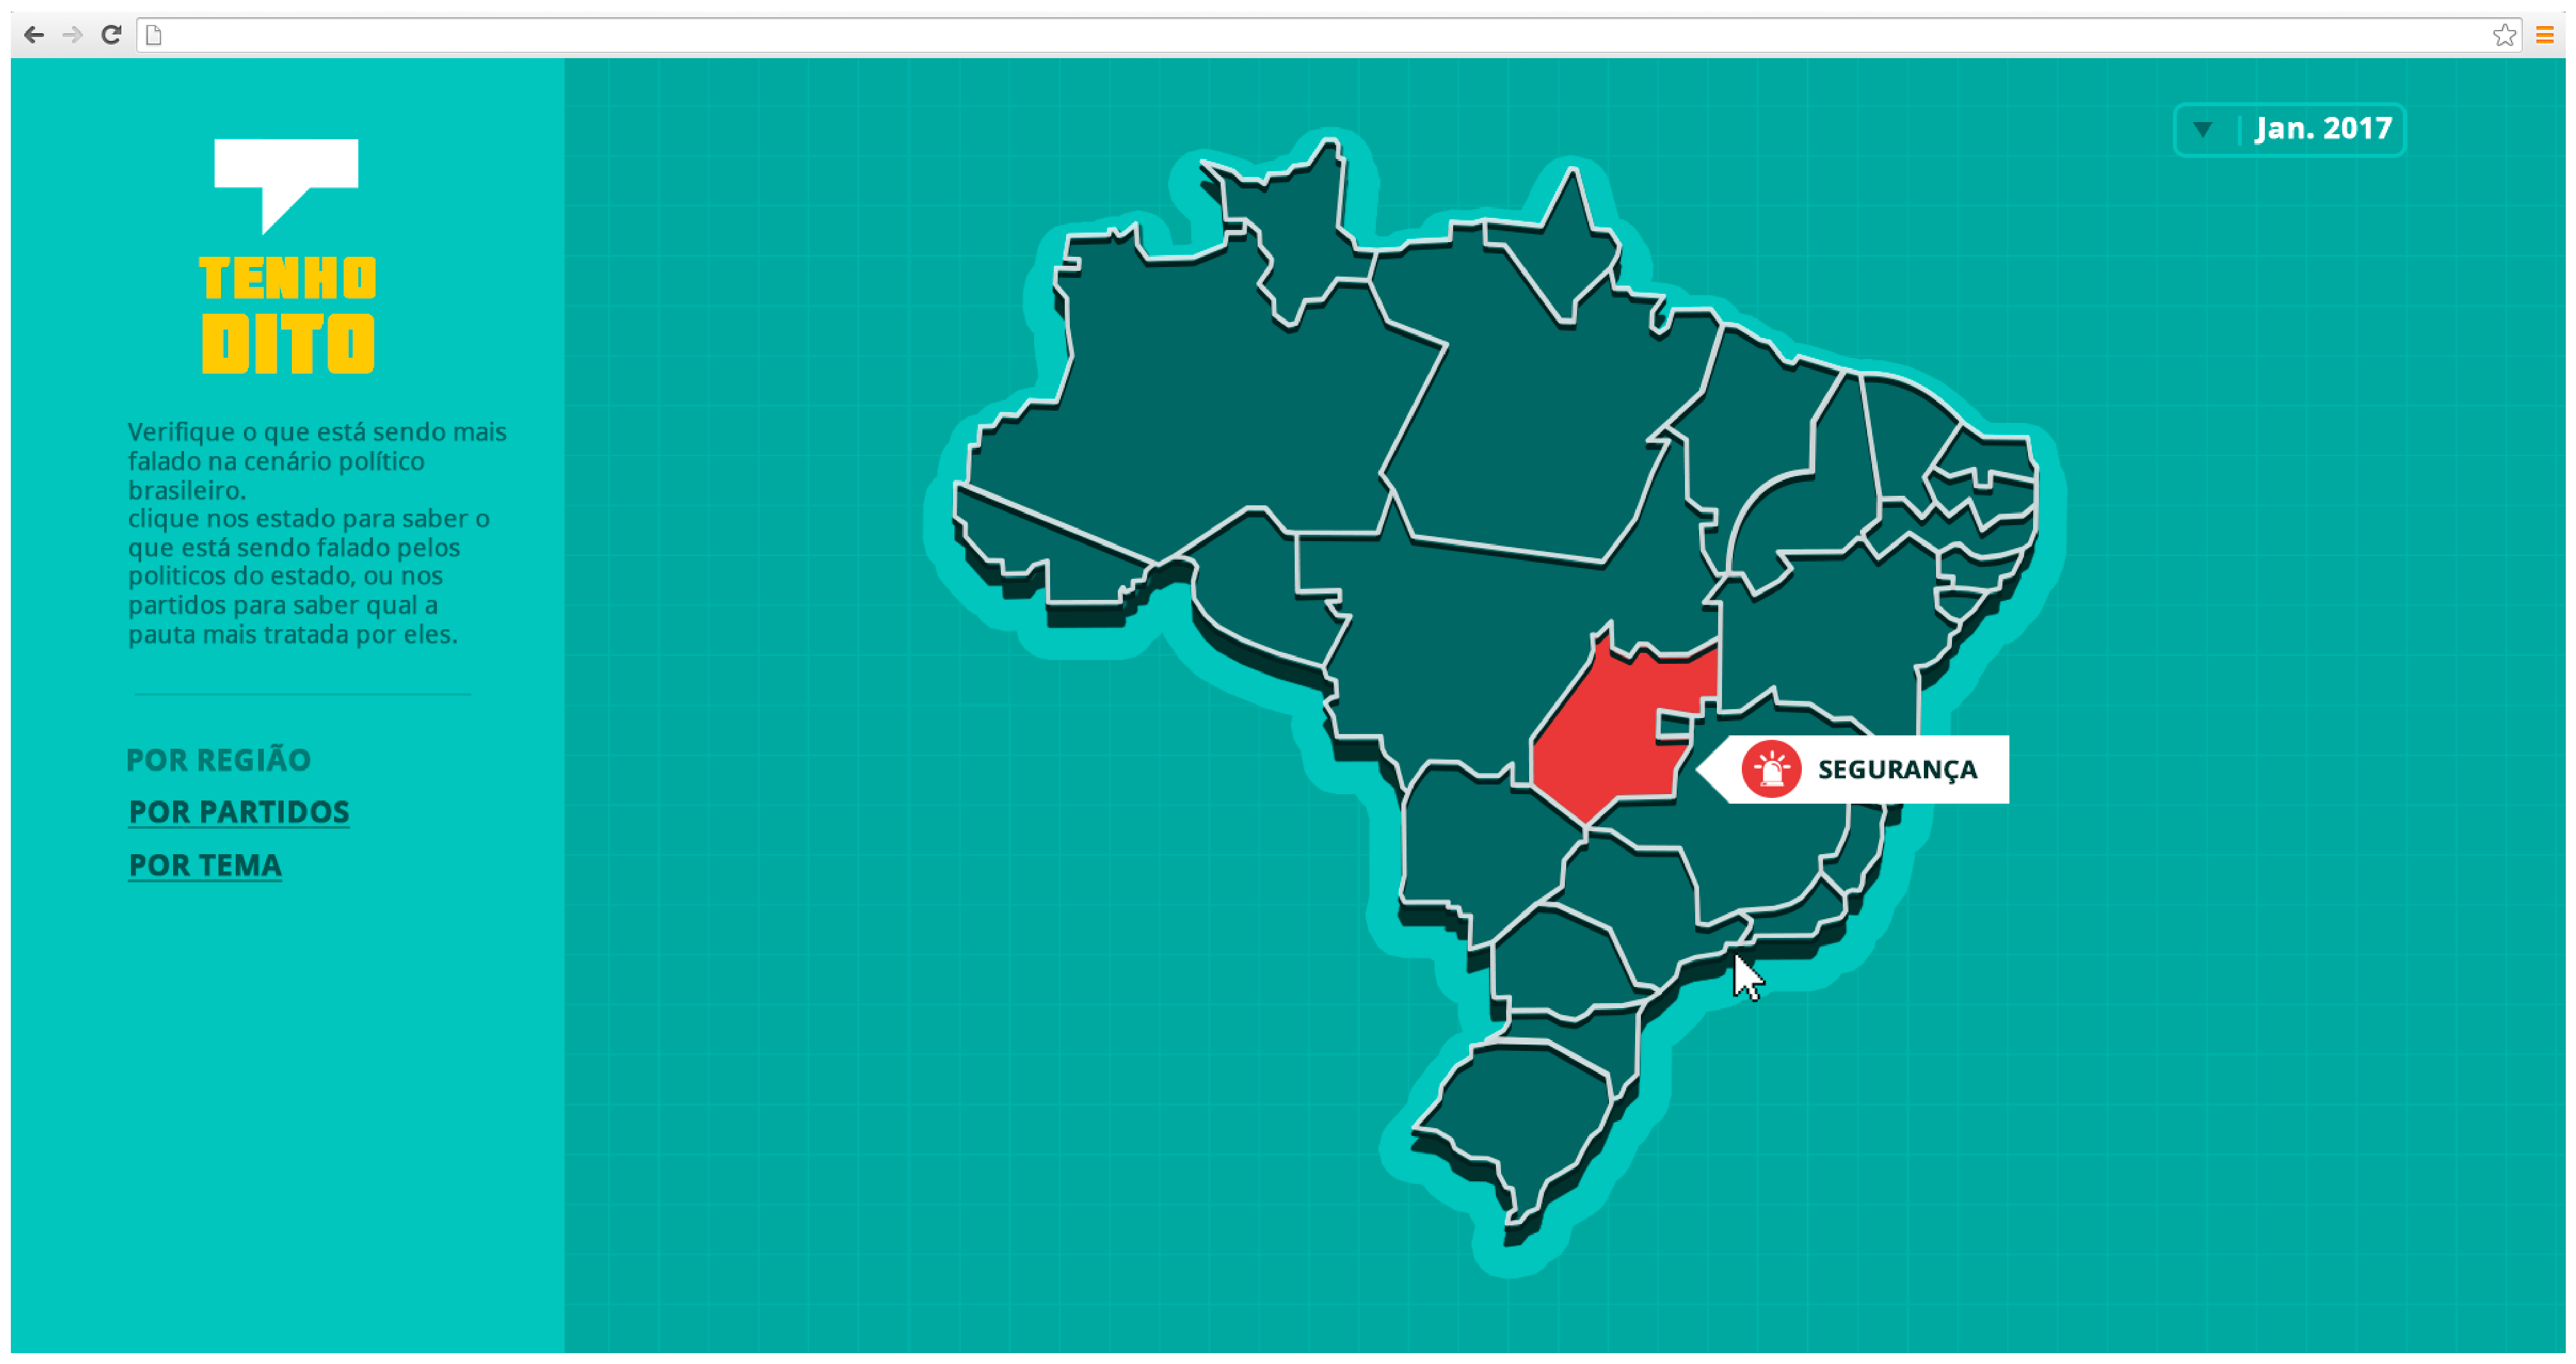
\includegraphics[scale=0.2]{figuras/tenhodito1.eps}
  \caption{Tela inicial do Tenho Dito - Visualização por região}
  \label{tenhodito1}
\end{figure}

Seguindo a abordagem por temas, ao clicar em um estado, o usuário é direcionado a outra página (figura \ref{tenhodito2}), onde encontra um gráfico de bolhas, detalhando os temas abordados pelos parlamentares do estado. Quanto maior a bolha, mais o tema foi abordado. Além disso, também são listados todos os deputados que representam aquele estado, juntamente com sua foto, partido e o tema predominante em seus discursos e proposições. Ainda não foram definidas as interações com o gráfico de bolhas.

\begin{figure}[h]
  \centering
  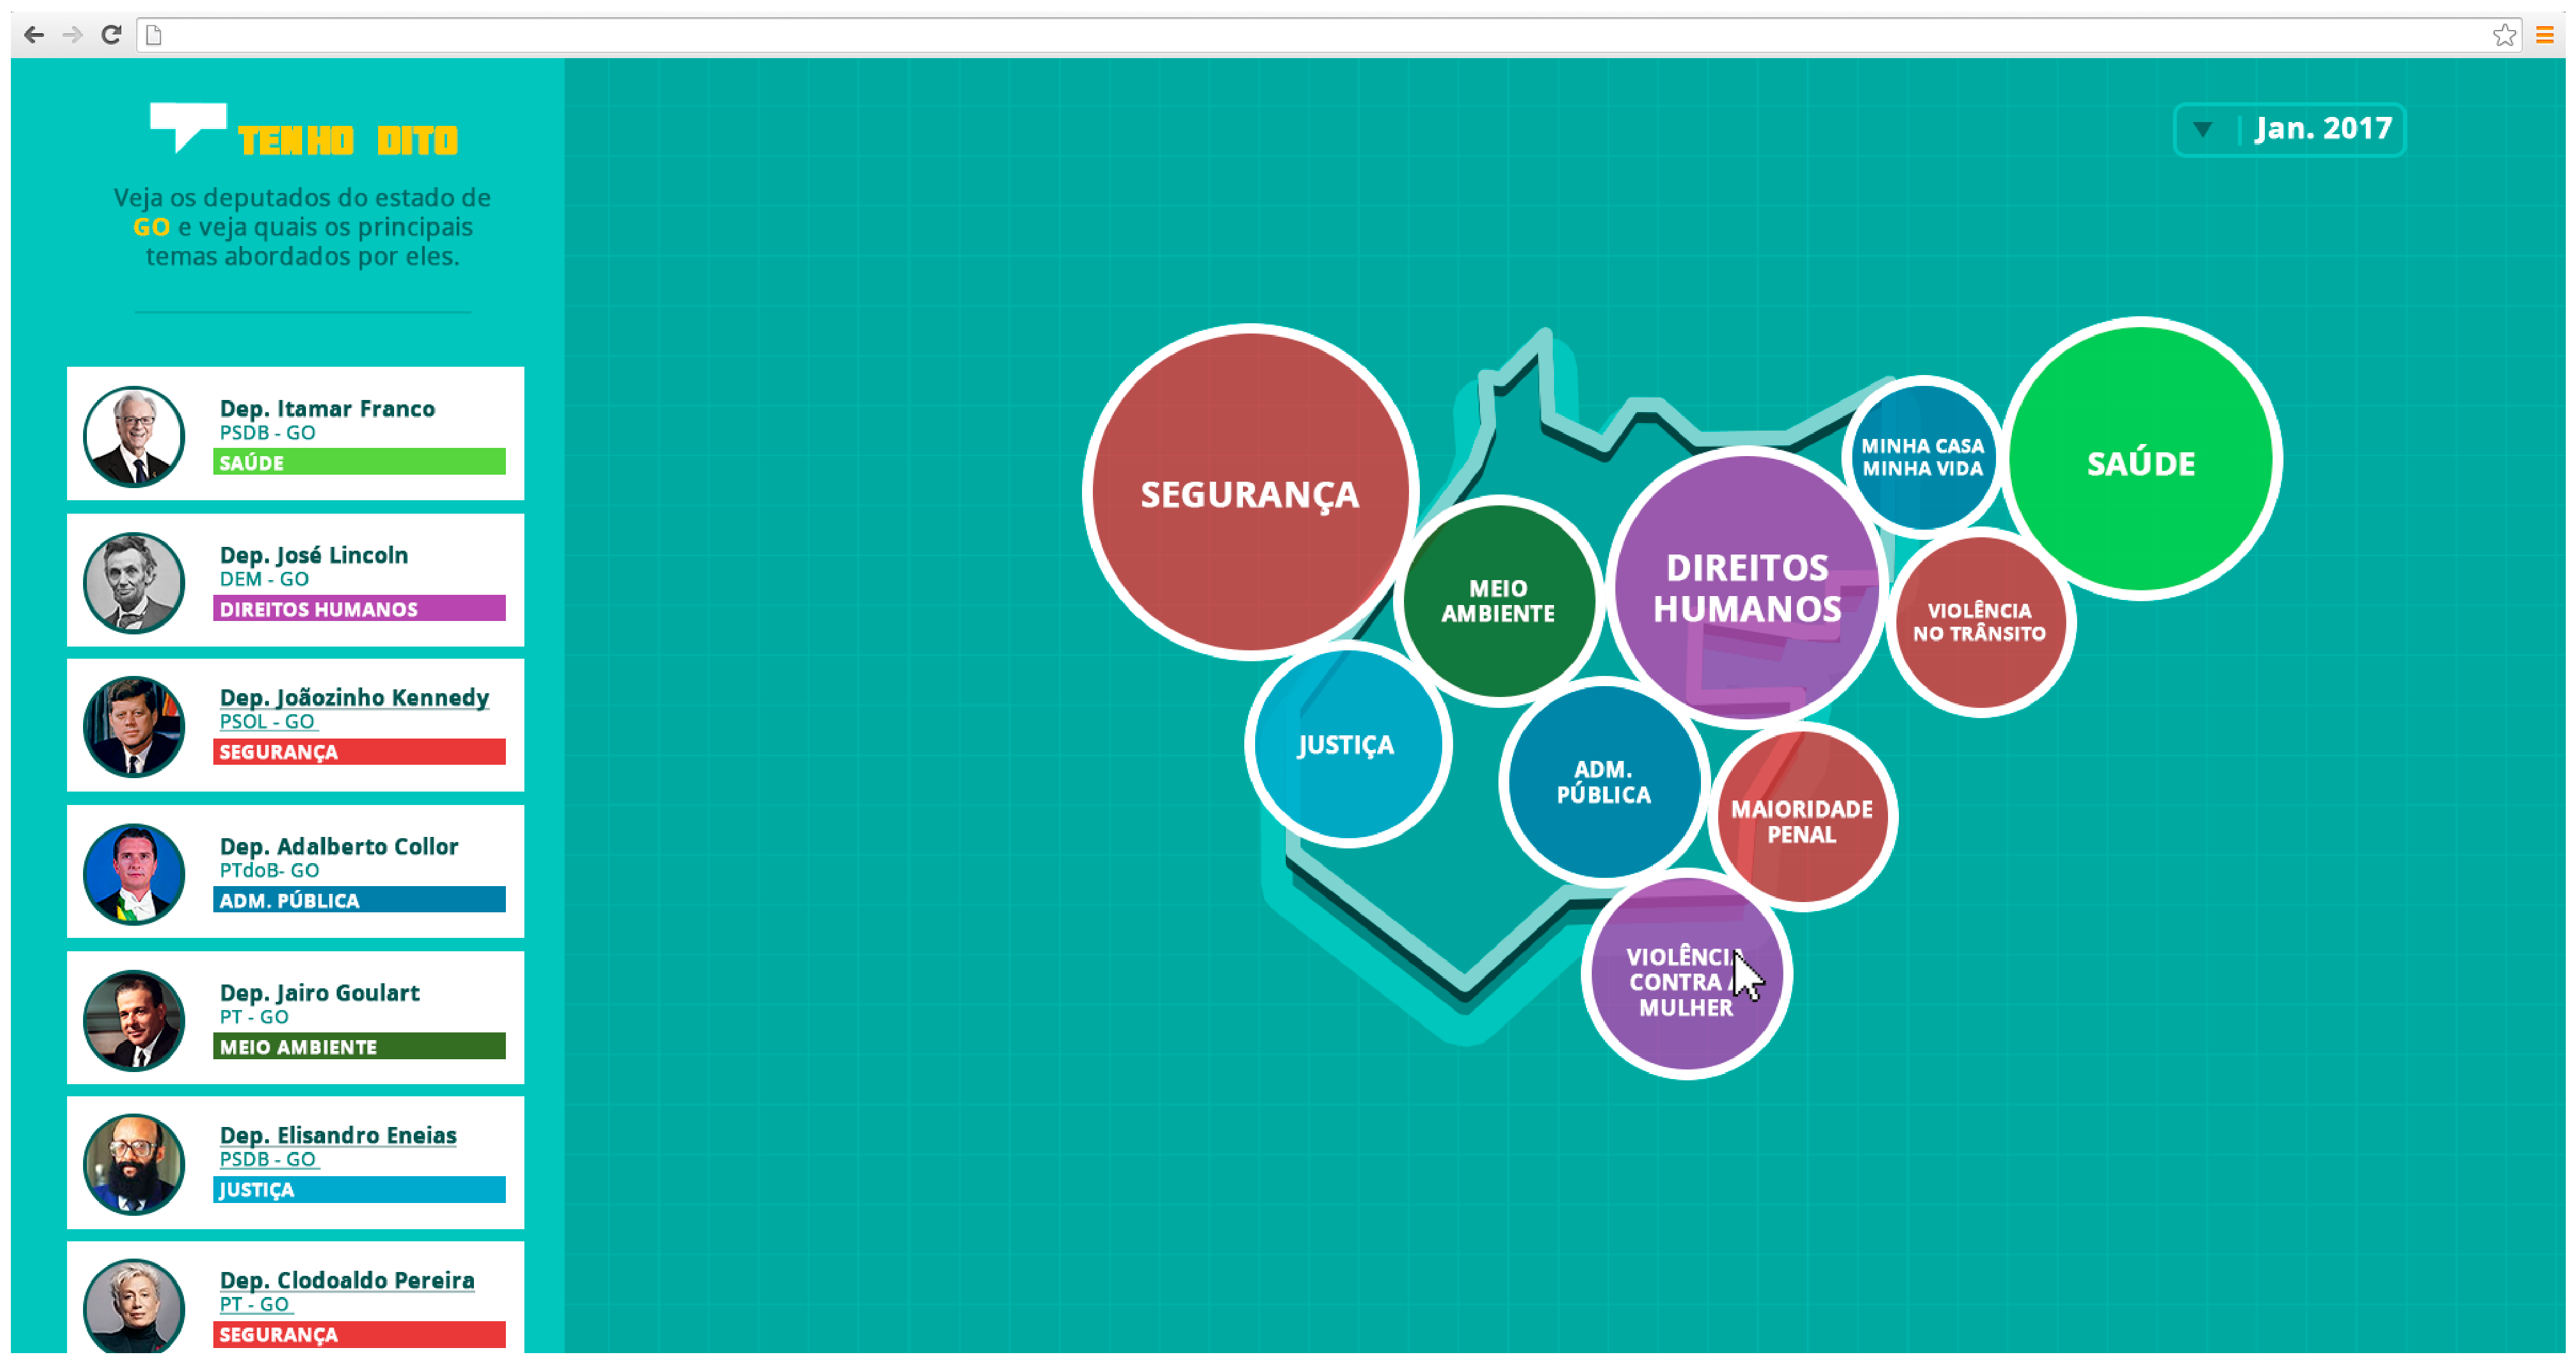
\includegraphics[scale=0.2]{figuras/tenhodito2.eps}
  \caption{Visualização detalhada dos temas, por região}
  \label{tenhodito2}
\end{figure}

O usuário também poderá selecionar um deputado específico e visualizar o seu perfil. Na tela de perfil do deputado (figura \ref{tenhodito3}), são exibidas as informações do deputado e também a quantidade de proposições e discursos analisados. Logo abaixo, será mostrado, dinâmica e randomicamente, trechos de discursos ou proposições e sua classificação. Além disso, serão listados todos os temas e a quantidade de discursos e proposições (por meio de gráfico de barras), com o objetivo de realizar uma comparação entre o que é mais dito pelo deputado e o que é mais proposto.

\begin{figure}[h]
  \centering
  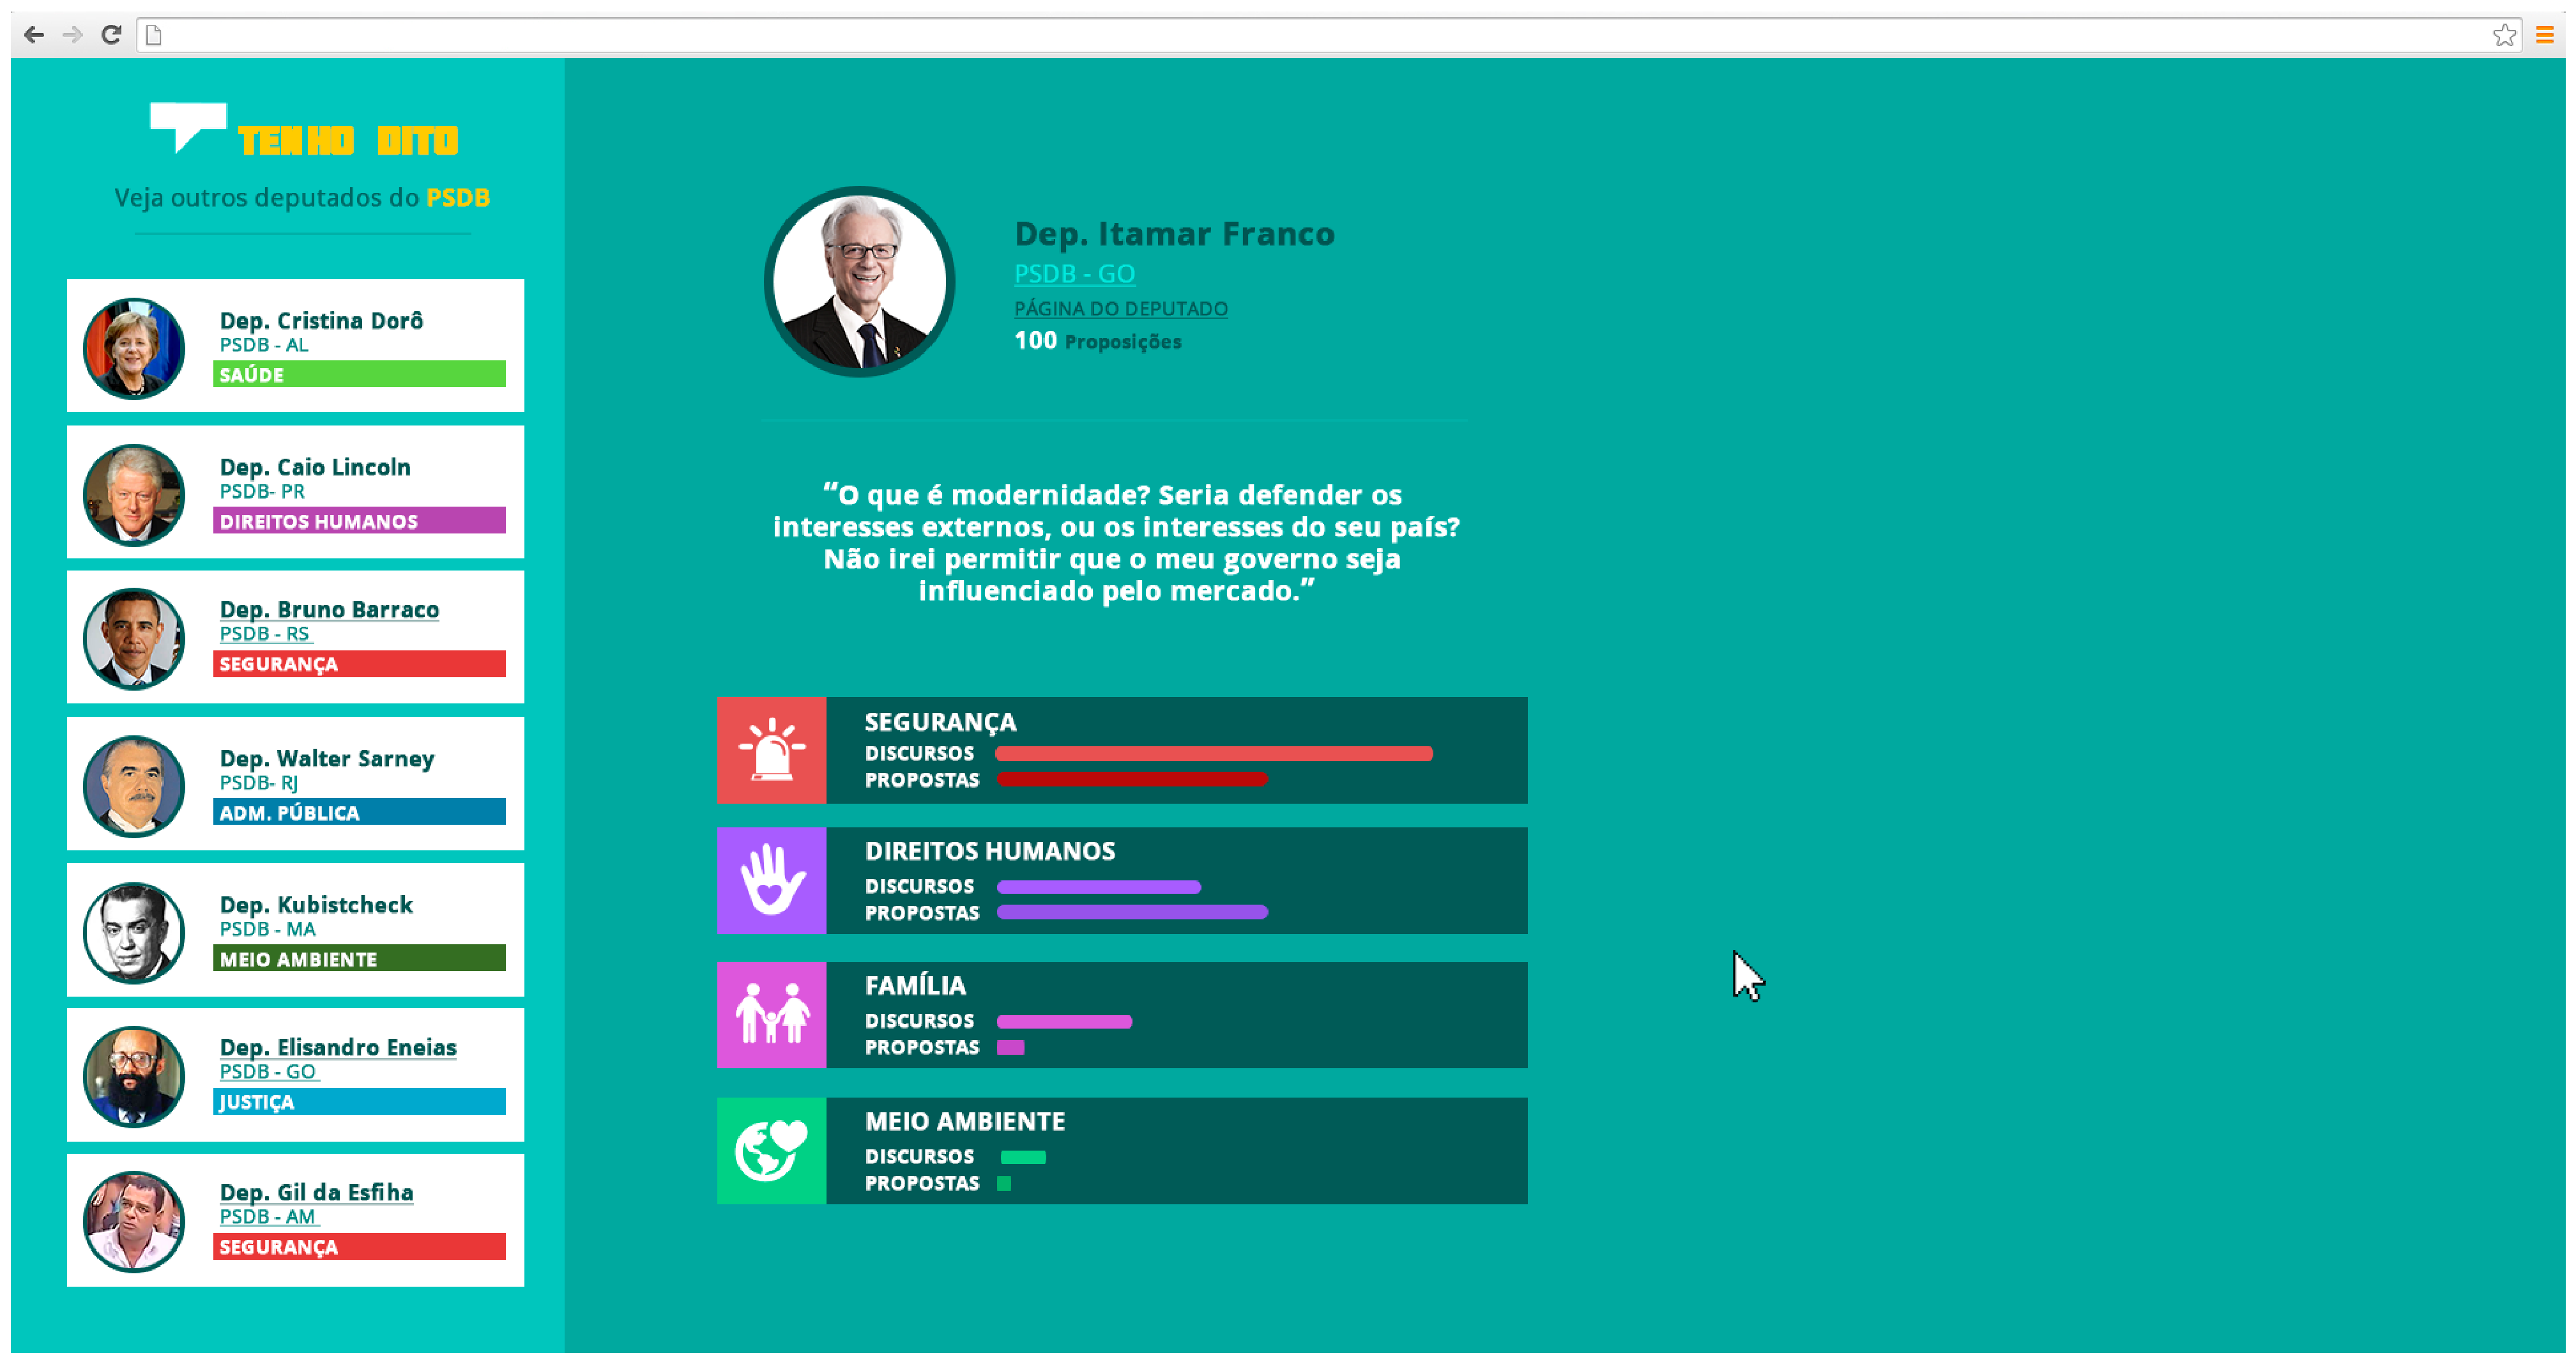
\includegraphics[scale=0.2]{figuras/tenhodito3.eps}
  \caption{Página de perfil do deputado}
  \label{tenhodito3}
\end{figure}

Quando o usuário clicar na opção de visualização por partidos, será exibida uma lista com os atuais partidos com representação na Câmara dos Deputados (figura \ref{tenhodito4}). O sitema possibilitará três tipos de ordenação: por tamanho (quantidade de deputados por partido), por ordem alfabética ou por tema. Nessa tela, também serão exibidos os temas mais abordados pelos partidos, através dos seus membros. Caso o partido tenho mais deputados cujo tema mais abordado em seus discursos e proposições é ``segurança'', por exemplo, o tema atribuído ao partido será ``segurança''.

\begin{figure}[h]
  \centering
  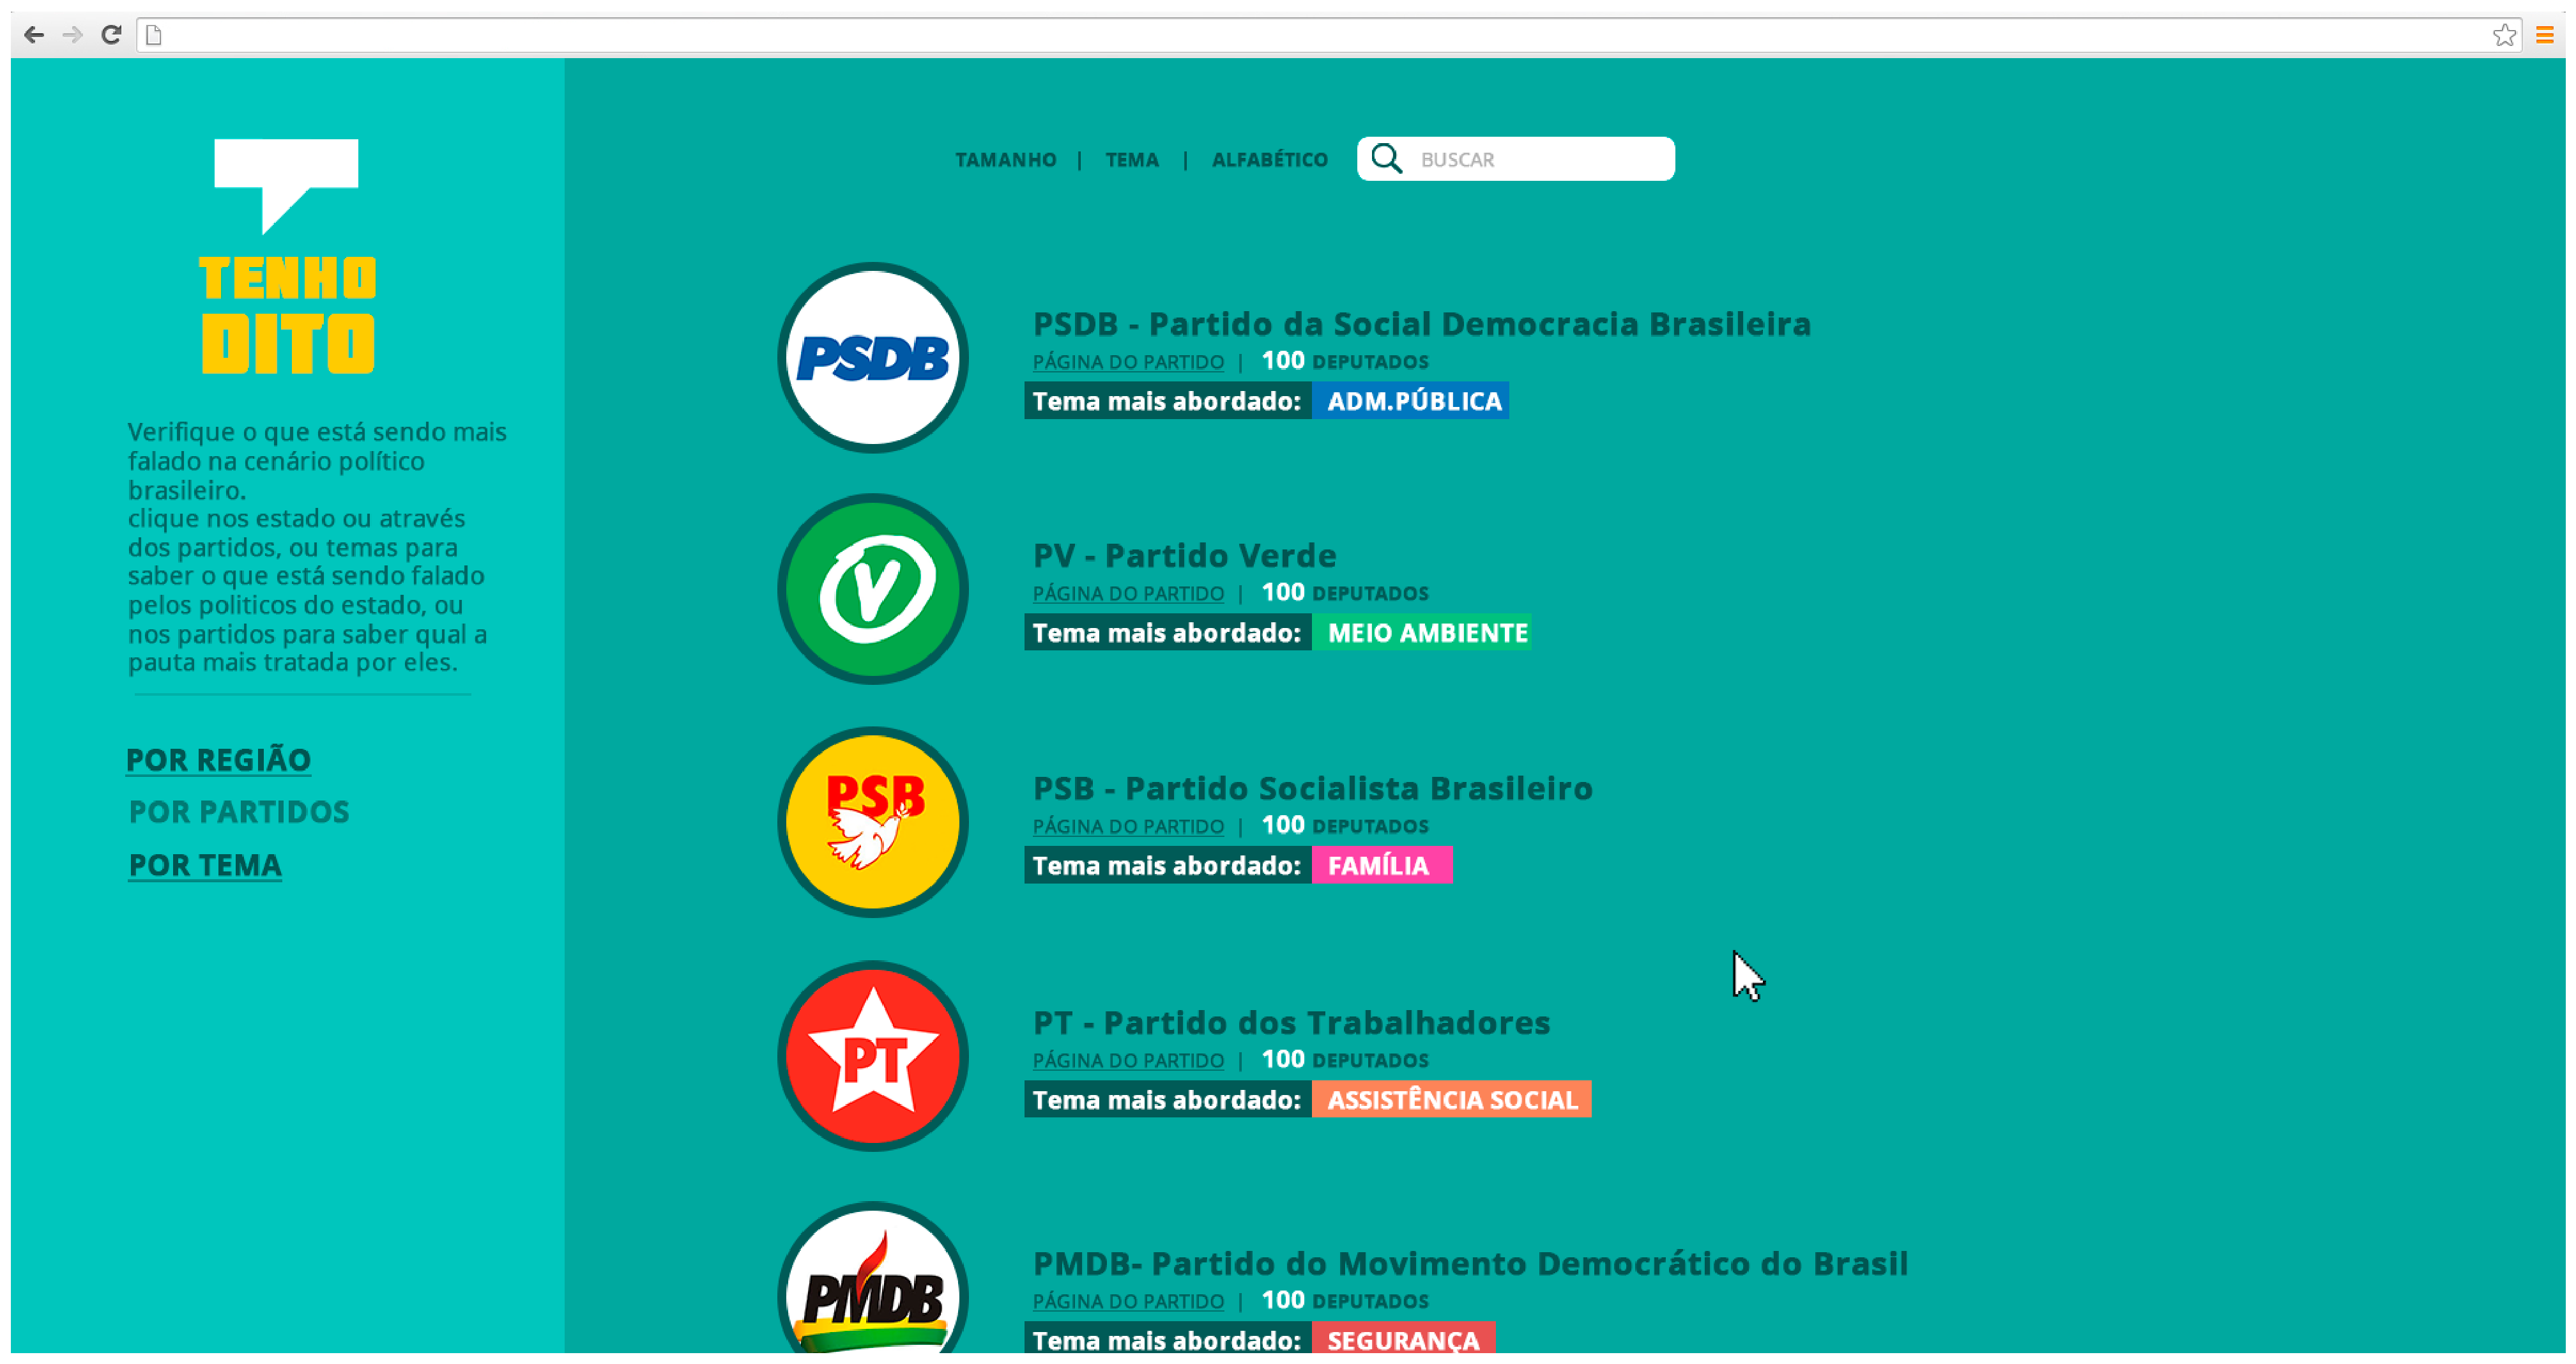
\includegraphics[scale=0.2]{figuras/tenhodito4.eps}
  \caption{Listagem dos partidos com representação na Câmara dos Deputados}
  \label{tenhodito4}
\end{figure}

O usuário poderá, assim como na abordagem por estado, escolher um partido para detalhar os temas abordados e, da mesma forma, é exibido um gráfico de bolhas com os temas abordados pelos deputados desse partido. Ao lado são mostrados todos os deputados do partido, independente do seu estado, ao clicar em algum deles o usuário é direcionado à pagina de perfil dele.

\begin{figure}[h]
  \centering
  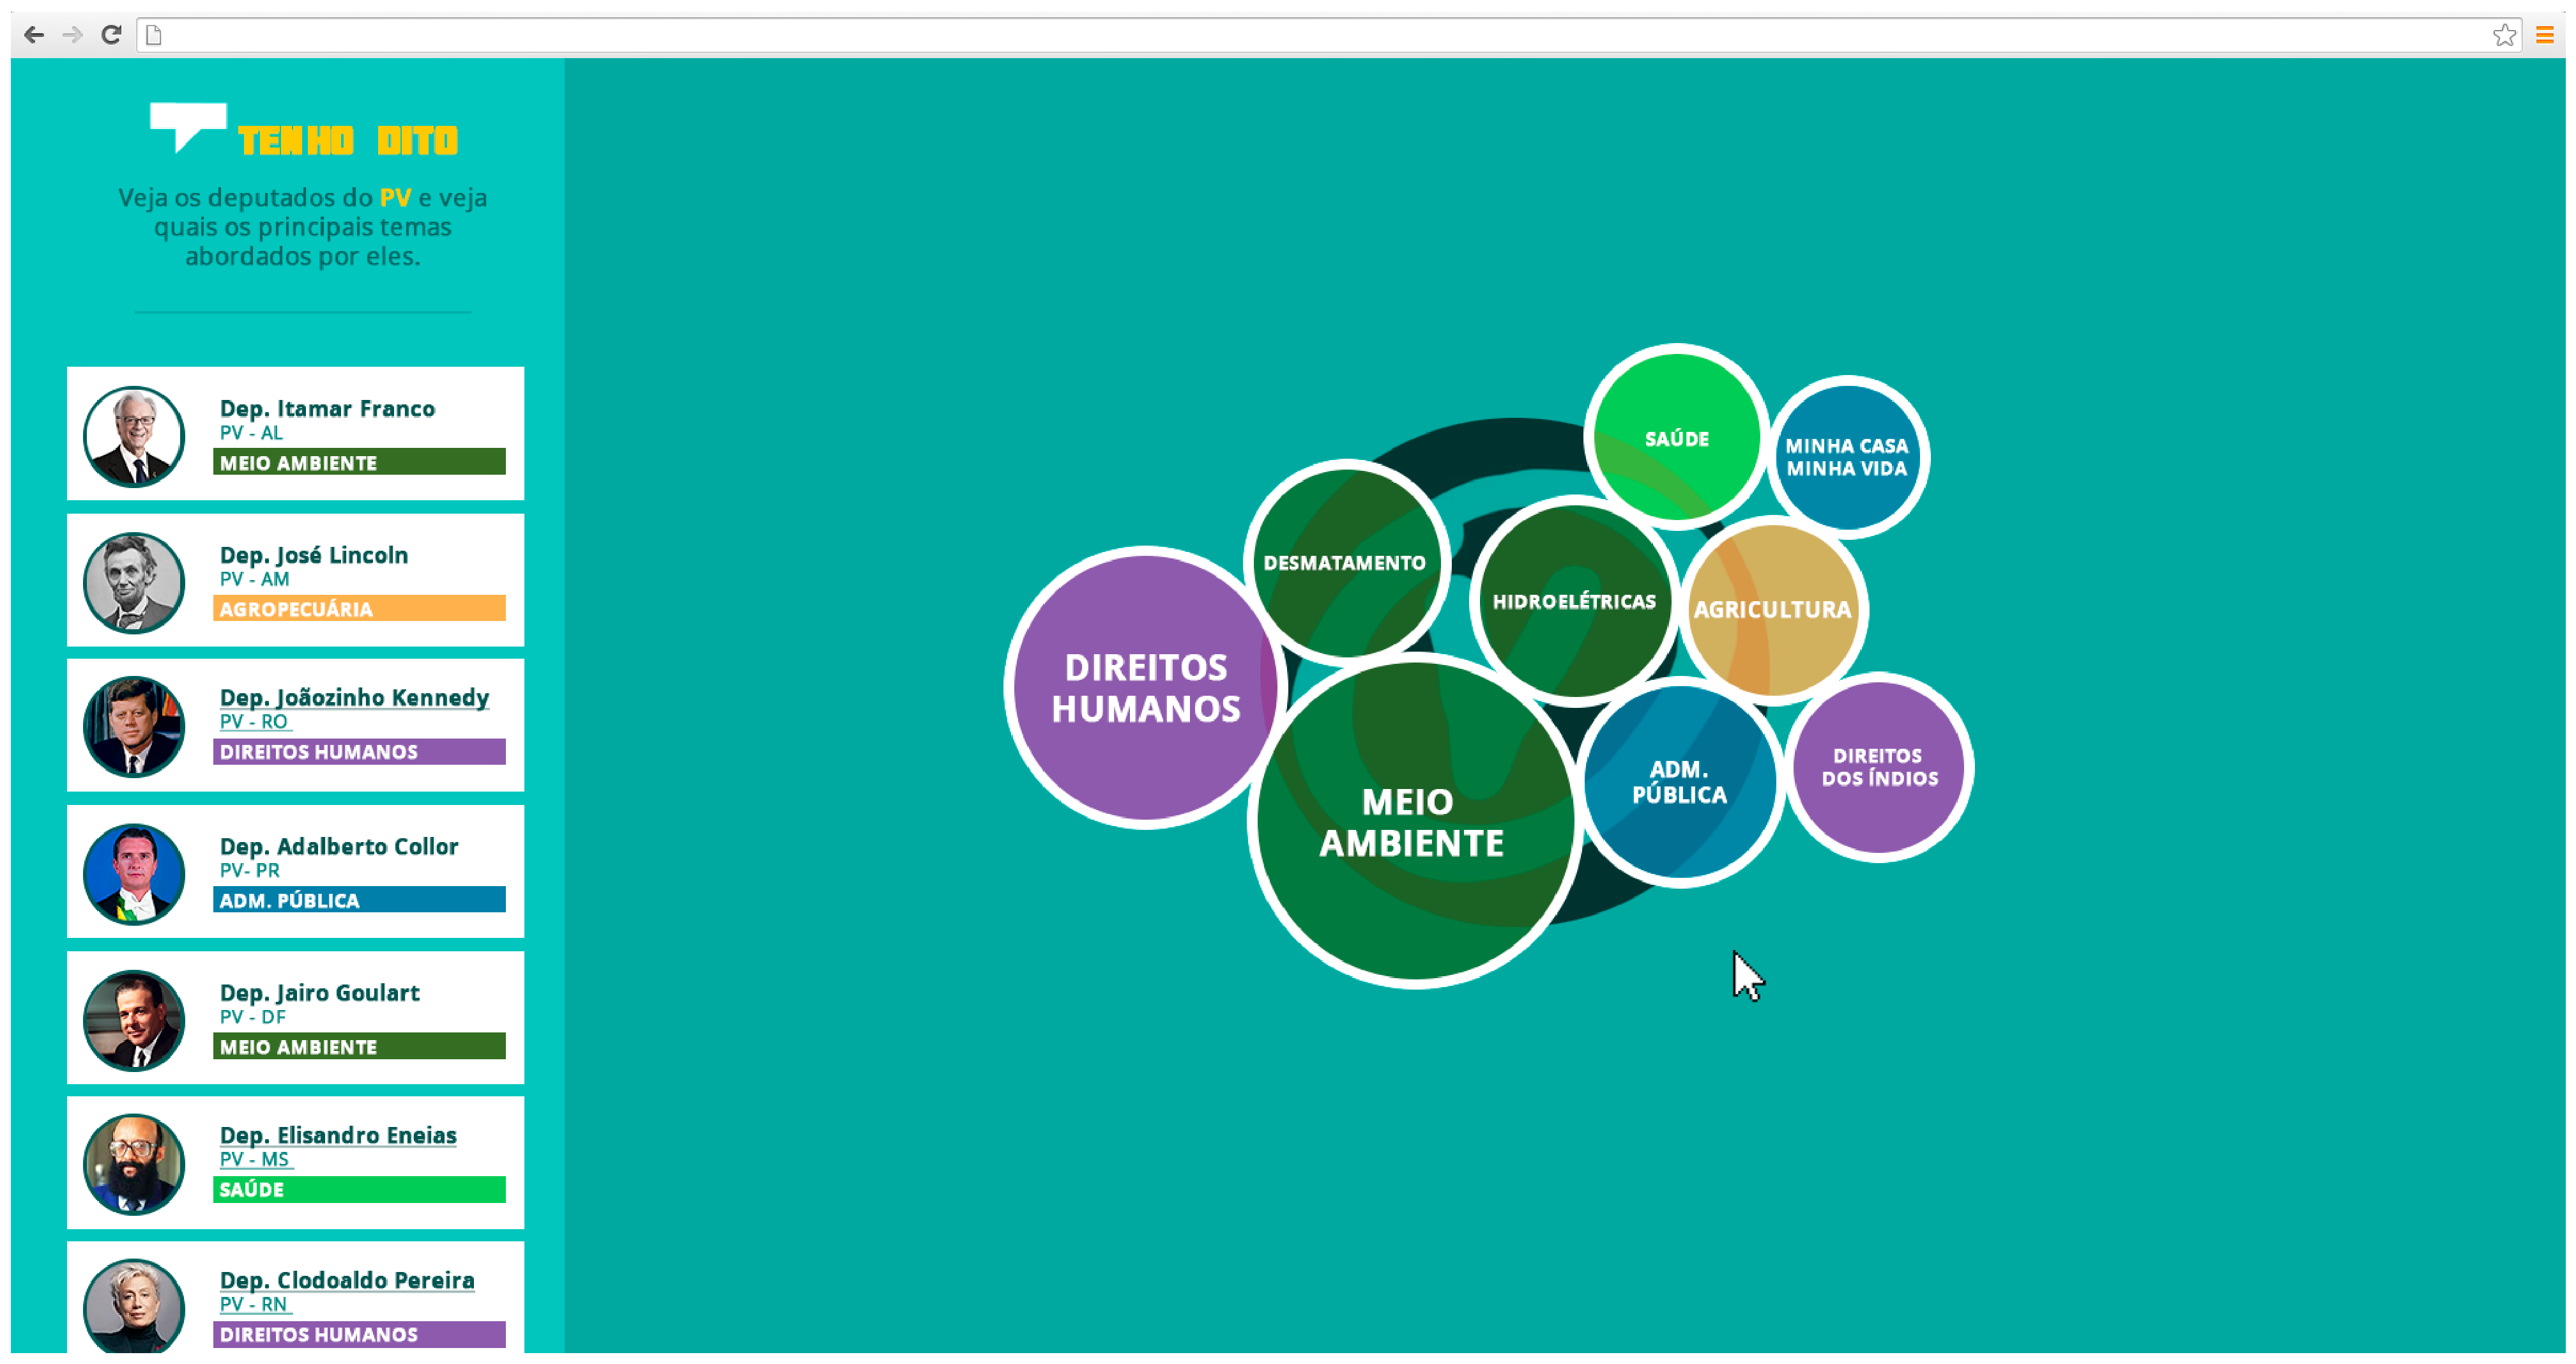
\includegraphics[scale=0.2]{figuras/tenhodito5.eps}
  \caption{Visualização detalhada dos temas, por partido}
  \label{tenhodito5}
\end{figure}

\chapter{\textit{Webservice} da Câmara dos Deputados}
\label{estrutura-webservice}

O \textit{webservice} atual (\textit{SOAP}) possui um total de 28 \textit{endpoints}, onde 5 são relacionados aos deputados, 9 aos órgãos, 9 às proposições e 5 às sessões e reuniões. A seguir descrevemos os \textit{endpoints} utilizados.

Os \textit{endpoints} que fornecem dados de deputados são:
\begin{itemize}
    \item \textbf{ObterDeputados:} retorna os deputados em exercício na Câmara dos Deputados
    \item \textbf{ObterDetalhesDeputado:} retorna detalhes dos deputados com histórico de participação em comissões, períodos de exercício, filiações partidárias e lideranças.
    \item \textbf{ObterLideresBancadas:} retorna os deputados líderes e vice-líderes em exercício das bancadas dos partidos
    \item \textbf{ObterPartidosCD:} retorna os partidos com representação na Câmara dos Deputados
    \item \textbf{ObterPartidosBlocoCD:} retorna os blocos parlamentares na Câmara dos Deputados.
\end{itemize}

Os \textit{endpoints} que fornecem dados de órgãos legislativos são:

\begin{itemize}
    \item \textbf{ListarCargosOrgaosLegislativosCD:} retorna a lista dos tipos de cargo para os órgãos legislativos da Câmara dos Deputados (ex: presidente, primeiro-secretário, etc)
    \item \textbf{ListarTiposOrgaos:} retorna a lista dos tipos de órgãos que participam do processo legislativo na Câmara dos Deputados
    \item \textbf{ObterAndamento:} retorna o andamento de uma proposição pelos órgãos internos da Câmara a partir de uma data específica
    \item \textbf{ObterEmendasSubstitutivoRedacaoFinal:} retorna as emendas, substitutivos e redações finais de uma determinada proposição
    \item \textbf{ObterIntegraComissoesRelator:} retorna os dados de relatores e pareces, e o link para a íntegra de uma determinada proposição
    \item \textbf{ObterMembrosOrgao:} retorna os parlamentares membros de uma determinada comissão
    \item \textbf{ObterOrgaos:} retorna a lista de órgãos legislativos da Câmara dos Deputados (comissões, Mesa Diretora, conselhos, etc.)
    \item \textbf{ObterPauta:} retorna as pautas das reuniões de comissões e das sessões plenárias realizadas em um determinado período
    \item \textbf{ObterRegimeTramitacaoDespacho:} retorna os dados do último despacho da proposição
\end{itemize}

Os \textit{endpoints} que fornecem dados de proposições são:

\begin{itemize}
    \item \textbf{ListarProposicoes:} retorna a lista de proposições que satisfaçam os critérios estabelecidos
    \item \textbf{ListarSiglasTipoProposicao:} retorna a lista de siglas de proposições
    \item \textbf{ListarSituacoesProposicao:} retorna a lista de situações para proposições
    \item \textbf{ListarTiposAutores:} retorna a lista de tipos de autores das proposições
    \item \textbf{ObterProposicao:} retorna os dados de uma determinada proposição a partir do tipo, número e ano
    \item \textbf{ObterProposicaoPorID:} retorna os dados de uma determinada proposição a partir do seu ID
    \item \textbf{ObterVotacaoProposicao:} retorna os votos dos deputados a uma determinada proposição em votações ocorridas no Plenário da Câmara dos Deputados
    \item \textbf{ListarProposicoesVotadasEmPlenario:} retorna todas as proposições votadas em plenário num determinado período
    \item \textbf{listarProposicoesTramitadasNoPeriodo:} retorna uma lista de proposições movimentadas em determinado período.
\end{itemize}

Os \textit{endpoints} que fornecem dados de sessões e reuniões são:

\begin{itemize}
    \item \textbf{ListarDiscursosPlenario:} retorna a lista dos deputados que proferiam discurso no Plenário da Cãmara dos Deputados em um determinado período.
    \item \textbf{ListarPresencasDia:} retorna a lista de presença de deputado em um determinado dia.
    \item \textbf{ListarPresencasParlamentar:} retorna as presenças de um deputado em um determinado período.
    \item \textbf{ListarSituacoesReuniaoSessao:} retorna a lista de situações para as reuniões de comissão e sessões plenárias da Câmara dos Deputados
    \item \textbf{ObterInteiroTeorDiscursosPlenario:} retorna o inteiro teor do discurso proferido no Plenário.
\end{itemize}

\chapter{Treinamento Inicial dos Classificadores}
\label{conjunto-palavras}

Para realizar o treinamento inicial dos classificadores \textit{naive} Bayes, é necessário fornecer um texto inicial e a sua classificação. Esse apêndice descreve os textos usados nesse trabalho para cada classificação.

\section{Classificação de Conteúdo Útil/Não-útil}

Para a classificação de ``conteúdo útil'' e ``conteúdo não-útil'', foram utilizadas os seguintes conjuntos de palavras iniciais:

\begin{itemize}
    \item \textbf{Conteúdo não-útil:} ``agradecimento agradeço muito obrigado v.exa. digníssimo nobre deputado amigo peço registro pela ordem pedir um aparte mérito emendas votado sessão comissão protocolo regimento pronunciamento divulgação''
    \item \textbf{Conteúdo útil:} ``educação universidade estudante professor ensino escola educador saúde médicos hospitais sus remédios atendimento hospitalar tratamento leitos religião templo igreja deus bíblia fé jesus segurança polícia crime violência punição arma contrabando ditadura militar golpe 31 de março tortura censura mulher aborto feminicídio feminismo feminista maria da penha petrobras pré-sal refinamento gasolina álcool combustível petrolão corrupção ministério público agu lava-jato mensalão impeachment crime de responsabilidade agronegócio agricultura agrícolas soja lavoura rural indústria desendustrialização empregos competitividade direitos humanos minorias tortura tráfego de pessoas trabalho escravo''
\end{itemize}

\section{Classificação Temática}

Para a classificação temática, os temas escolhidos e seus respectivos conjuntos de palavras utilizados foram:

\begin{itemize}
    \item \textbf{Agropecuária:} ``agropecuária fertilizantes agronegócio abate suínos ovos cabeças bovinos frangos exportação carne animal milho ração aviária laranja safra frutos pomares laranjeiras fazenda pés produzir hectares quilos fruta  produtor orgânico consumidor toneladas  embrapa bezerros pecuária veterinária filhotes sementes agro produção água sol área degradação produtor café importação agrícola pescador alimento alimentação açúcar ibge fertilizante lavouras grão bovino soja etanol frutos rural''
    \item \textbf{Saúde:} ``saúde médico doença vírus zika pesquisa paciente estudo mosquito epidemia chikungunya tratamento procedimento tremor causa gêmeos dengue transmissão cubano bebês cirurgia cientista risco sintomas dor ultrassom dr aegypt ovário microcefalia gravidez sistema imune imunológico drogas fertilização febre diagnóstico renal sangue insuficiente insuficiência cérebro idade nascimento hipotálamo morte dna corpo cardio muscular vacina''
    \item \textbf{Esporte:} ``esporte jogo jogador clube time contrato treino mundial atleta surf futebol disputa penalidade compo estádio ataque atacante bola goleiro treinador seleção técnico campeonato gol pontuação futsal vitória perde perdedor lutador torcedor torcida rival diretor falta conquista prorrogação empate surfista assistência ufc''
    \item \textbf{Educação:} ``educação estudo ensino escola médio prova enem universidade faculdade matemática avaliação aluno curso pesquisa inep exame pública mec professor redação criança texto reforma currículo curricular campus leitura literatura desempenho formação qualidade disciplina fies superior analfabeto analfabetismo português física química geometria''
    \item \textbf{Ciência e Tecnologia:} ``ciência tecnologia novidades empresa startup smart serviço smartphone consumidor produto google aparelho samsung celular internet inteligência artificial desenvolvimento dispositivo lançamento  aplicativo inovar inovação sony conectar conectado comunicação 3g 4g 5g iphone sistema telecomunicações satélite design científico artigo computador tráfego eletrônico apple whatsapp televisão tv telefone avanço espacial''
    \item \textbf{Economia:} ``economia trabalho crédito compra banco bilhões milhões vendas contas inflação consumidor juros queda crise taxa resultado econômico gasto pagamento valor financeiro investimento dinheiro índice comércio empresa desemprego fgts limite emprego cartão varejo déficite fundo recessão recuo salário lojista tesouro fiscal inadimplente recurso dólar euro moeda bolsa endividado projeções crescimento capital ações negócios''
    \item \textbf{Política:} ``política deputado congresso pt partido estado união reforma lei legislatura legislação pec pmdb aprovar voto bancada população senado senador câmara deputado sindicato candidato candidatura mandato comissão ministério constituição eleição eleições delação judiciário votações prefeitura prefeito vereador assembleia procurador corrupção''
    \item \textbf{Meio Ambiente:} ``ambiente área água rio empresa desastres multa seca barragem furacão desmatamento floresta tropical ibama parque preservação região terra planeta poluição ambiental espécie animais plantas platações petróleo emissão gás chuva temporal sol clima temperatura estufa aquecimento global umidade terremoto planeta biodiversidade biologia mar oceano calor energia sustentável madeira reflorestamento tempestade niño florescimento hídrico climática''
    \item \textbf{Direitos Humanos:} ``direitos humanos mulher tortura violência morte justiça onu sexual vítima sexual adolescente presídio prevenção união negro branco segurança refugiado homens humanitario conflito sociedade racismo sexismo machismo machista feminismo feminista defensoria estupro jovens criança prostituição assassinato liberdade idoso inclusão social preconceito gay homossexual heterosexual lgbt lésbica bissexual travesti transexual transgênero impunidade imigrante''
    \item \textbf{Segurança:} ``segurança ataque polícia suspeito morte crime terror rebelde investigação civil federal guerra onu vítima invasão preso presídio assassinato bombardeio apreensão incidente defesa exército marinha aeronáutica prisão ameaça bomba testemunha promotor policial tragédia assalto protesto''
\end{itemize}


\end{apendicesenv}

% \input{editaveis/anexos}
\printindex

\end{document}

